\documentclass[11pt]{book}

\RequirePackage{silence}
\WarningFilter{remreset}{The remreset package}

\title{MAT223 - Linear Algebra}
\author{Callum Cassidy-Nolan}

% Packages
\usepackage{amsmath}
\usepackage{amssymb}
\usepackage{mathtools}
\usepackage{xcolor}
\usepackage{amsthm}
\usepackage{thmtools}
\usepackage{amsfonts}
\usepackage{geometry}
\usepackage{gauss}
\usepackage{pifont}
\usepackage{hyperref}
\usepackage{witharrows}
\usepackage{cleveref}
\usepackage{tikz}
\usepackage{bm}
\usepackage{todonotes}
\usepackage{enumitem}
\usepackage{mdframed}
\usetikzlibrary{patterns,angles,quotes,decorations.pathreplacing}
\hypersetup{
    colorlinks=true, %set true if you want colored links
    linktoc=all,     %set to all if you want both sections and subsections linked
    linkcolor=blue,  %choose some color if you want links to stand out
}


% BlackSquare for proofs
\renewcommand{\qedsymbol}{$\blacksquare$}

\theoremstyle{definition}

% Matricies
\newcommand\mat[2][b]{\begin{#1matrix}#2\end{#1matrix}}

% Augmented matrix
\makeatletter
\renewcommand*\env@matrix[1][*\c@MaxMatrixCols c]{%
  \hskip -\arraycolsep
  \let\@ifnextchar\new@ifnextchar
  \array{#1}}
\makeatother

% Modular Arithmetic
\newcommand{\Mod}[1]{\ (\mathrm{mod}\ #1)}

% Automatic Parenthesis scaling
\delimitershortfall-1sp
\usepackage{mleftright}
\mleftright % make \left & \right behave like \mleft & \mright

% Theorems
\newtheoremstyle{break}
  {\topsep}{\topsep}%
  {\itshape}{}%
  {\bfseries}{}%
  {\newline}{}%

\theoremstyle{break}

\newtheorem{remark}{Remark}[section]

\newtheorem{ver}{Verfication}[section]

\newtheorem{ex}{Exercise}[section]

\newtheorem{eg}{Example}[section]

% definition env
\newmdtheoremenv{defn}{Definition}

% Note env
\newmdtheoremenv{nt}{Note}

% definition env no num
\newtheorem*{defnnonum}{Definition}

% theorem envs
\newtheorem{thm}{Theorem}

% theorem envs without counter

\newtheorem{propo}[thm]{Proposition}

\newtheorem{crly}[thm]{Corollary}

\newtheorem{lemma}[thm]{Lemma}

\newtheorem{axiom}[thm]{Axiom}

\newtheorem*{thmnonum}{Theorem}

\newtheorem*{propononum}{Proposition}

\newtheorem*{crlynonum}{Corollary}

\newtheorem*{lemmanonum}{Lemma}

\newtheorem*{axiomnonum}{Axiom}


\newtheorem{note}{Note}[section]

\newtheorem{mnote}[note]{Note}

\newtheorem*{notation}{Notation}
    % warning env
\newtheorem*{warning}{Warning}

% So todo's don't get cut off
\setlength{\marginparwidth}{3cm}

% Define cuboids
\tikzset{
  annotated cuboid/.pic={
    \tikzset{%
      every edge quotes/.append style={midway, auto},
      /cuboid/.cd,
      #1
    }
    \draw [every edge/.append style={pic actions, densely dashed, opacity=.5}, pic actions]
    (0,0,0) coordinate (o) -- ++(-\cubescale*\cubex,0,0) coordinate (a) -- ++(0,-\cubescale*\cubey,0) coordinate (b) edge coordinate [pos=1] (g) ++(0,0,-\cubescale*\cubez)  -- ++(\cubescale*\cubex,0,0) coordinate (c) -- cycle
    (o) -- ++(0,0,-\cubescale*\cubez) coordinate (d) -- ++(0,-\cubescale*\cubey,0) coordinate (e) edge (g) -- (c) -- cycle
    (o) -- (a) -- ++(0,0,-\cubescale*\cubez) coordinate (f) edge (g) -- (d) -- cycle;
    \path [every edge/.append style={pic actions, |-|}]
    (b) +(0,-5pt) coordinate (b1) edge ["\cubex \cubeunits"'] (b1 -| c)
    (b) +(-5pt,0) coordinate (b2) edge ["\cubey \cubeunits"] (b2 |- a)
    (c) +(3.5pt,-3.5pt) coordinate (c2) edge ["\cubez \cubeunits"'] ([xshift=3.5pt,yshift=-3.5pt]e)
    ;
  },
  /cuboid/.search also={/tikz},
  /cuboid/.cd,
  width/.store in=\cubex,
  height/.store in=\cubey,
  depth/.store in=\cubez,
  units/.store in=\cubeunits,
  scale/.store in=\cubescale,
  width=10,
  height=10,
  depth=10,
  units=cm,
  scale=.1,
}

% highlighting shortcuts
\newcommand{\hlimpo}[1]{\textcolor{red}{\textbf{#1}}}
\newcommand{\hlwarn}[1]{\textcolor{yellow}{\textbf{#1}}}
\newcommand{\hldefn}[1]{\textcolor{blue}{\index{#1}\textbf{#1}}}
\newcommand{\hlnotea}[1]{\textcolor{green}{\textbf{#1}}}
\newcommand{\hlnoteb}[1]{\textcolor{cyan}{\textbf{#1}}}
\newcommand{\hlb}[2]{\colorbox{#1!30!background}{#2}}
\newcommand{\hlbnotea}[1]{\hlb{green}{#1}}
\newcommand{\hlbnoteb}[1]{\hlb{cyan}{#1}}
\newcommand{\hlbnotec}[1]{\hlb{yellow}{#1}}
\newcommand{\hlbnoted}[1]{\hlb{magenta}{#1}}
\newcommand{\hlbnotee}[1]{\hlb{red}{#1}}
\newcommand{\WTP}{\textcolor{bwhite}{WTP} }
\newcommand{\WTS}{\textcolor{bwhite}{WTS} }



\begin{document}

\maketitle

\tableofcontents

\renewcommand{\listtheoremname}{List of Definitions}
\listoftheorems[ignoreall,show={defn}]


\renewcommand{\listtheoremname}{\textsl{List of Theorems}}
\listoftheorems[ignoreall,
show={axiom,lemma,thm,crly,propo}
]


\chapter{Week 9}%
\label{chp:week_9}
% chapter week_9

Linear transformations and such

\section{Linear Transformations}%
\label{sec:linear_transformations}
% section linear_transformations

\begin{defn}[Linear Transformation]\index{Linear Transformation}\label{defn:linear_transformation}
    Let $V$ and $W$ be subspaces. A function $\mathcal{T} : V \to W $ is called
    a linear transformation if for all $\vec{u}, \vec{v} \in V$ and $a \in \mathbb{R}$ it satisfies
    \begin{enumerate}
        \item $\mathcal{T}(\vec{u} + \vec{v}) = \mathcal{T}(\vec{u}) + \mathcal{T}(\vec{v})$ 
        \item $\mathcal{T}(a \vec{u}) = a \mathcal{T}(\vec{u})$ 
    \end{enumerate}
\end{defn}

%TODO: Prove those two properties hold

\begin{thm}[Unique Matrix for LT's]\index{Unique Matrix for LT's}\label{thm:unique_matrix_for_lt_s}
    For any linear transformation $L : V \to W $ there is a matrix $A$  such that $L\left(\vec{x}\right) = A\vec{x}$ for all $\vec{x} \in V$ 
\end{thm}

\begin{eg}
    We'll show that $\mathcal{R}$ is a linear transformation where $\mathcal{R}$
    is a counter clockwise rotation of $\frac{\pi }{2}$ radians
    \begin{equation*}
       \mathcal{R}\left(\mat{ x \\ y }\right) = \mat{ 0 & -1 \\ 1 & 0 } \mat{ x \\ y }
    \end{equation*}
    Let $\vec{u}, \vec{v} \in \mathbb{R}^2$ we know that for some $x_1, y_1,
    x_2, y_2 \in \mathbb{R}$ that
    \begin{equation*}
        \vec{u} = \mat{ x_1 \\ y_1 } \text{ and } \vec{v} = \mat{ x_2 \\ y_2 }
    \end{equation*}
    \begin{align*}
        \mathcal{R}\left(\mat{ x_1 \\ y_1 }\right) + \mathcal{R}\left(\mat{ x_2
        \\ y_2 }\right) &= \mat{ -y_1 \\ x_1 } + \mat{ -y_2 \\ x_2 }\\
                        &= \mat{ - \left( y_1 + y_2 \right) \\ x_1 + x_2 }\\
    \end{align*}
    Which is exactly equal to $\mathcal{R}\left(\vec{u} + \vec{v}\right)$ as
    required, then let $\alpha \in \mathbb{R}$ and we know that
    \begin{equation*}
        \mathcal{R}\left(\alpha \vec{u}\right) = \mat{ -\alpha y_1 \\ \alpha x_1 }
    \end{equation*}
    But also that 
    \begin{equation*}
        \alpha \mathcal{R}\left(\vec{u}\right) = \mat{ -\alpha y_1 \\ \alpha x_1 }
    \end{equation*}
    So then we've shown that $\mathcal{R}\left(\alpha \vec{u}\right) = \alpha
    \mathcal{R }\left(\vec{u}\right)$ but also that $\mathcal{R}\left(\vec{u} + \vec{v}\right) = \mathcal{R}\left(\vec{u}\right) + \mathcal{R}\left(\vec{v}\right)$ as req'd
\end{eg}

\begin{eg}
    We'll show that $\mathcal{T} : \mathbb{R}^2 \to \mathbb{R}^2 $ where
    $\mathcal{T} \mat{ x \\ y } = \mat{ x + 2 \\ y }$ is not a linear
    transformation.

    Let $\vec{j} = \mat{ 0 \\ 0 }, \vec{k} = \mat{ 0 \\ 0 }$ we have that
    \begin{equation*}
        \mathcal{T}(\mat{ 0 \\ 0 } + \mat{ 0 \\ 0 }) = \mat{ 2 \\ 0 }       
    \end{equation*}
    But then we can see that 
    \begin{equation*}
        \mathcal{T}(\mat{ 0 \\ 0 }) + \mathcal{T}(\mat{ 0 \\ 0 }) = \mat{ 2 \\ 0
        } + \mat{ 2 \\ 0 } = \mat{ 4 \\ 0 }         
    \end{equation*}
    Then we conclude that $\mathcal{T}(\vec{j} + \vec{k}) \neq
    \mathcal{T}(\vec{j}) + \mathcal{T}(\vec{k})$ 
\end{eg}

\begin{eg}
    We'll show that $\mathcal{P}$ is a linear transformation 
    n
    \begin{note}
        We'll show that it is closed under addition and multiplication
    \end{note}
    \begin{equation*}
        \mathcal{P}(\mat{ x \\ y }) = \mathit{comp}_{\vec{u}} {\mat{ x \\ y }} 
    \end{equation*}
    Let $\vec{j}, \vec{k} \in \mathbb{R}^2$ we know that 
    \begin{equation*}
        \mathit{comp}_{\vec{u}} {\vec{j}}  = \left( \frac{\vec{u} \cdot
        \vec{j}}{\left\Vert \vec{u} \right\Vert^2} \right) \vec{u} \text{ and }
        \mathit{comp}_{\vec{u}} {\vec{k}}  = \left( \frac{\vec{u} \cdot
        \vec{k}}{\left\Vert \vec{u} \right\Vert^2} \right) \vec{u}
    \end{equation*}
    And thus their product yields
    \begin{align*}
        \mathit{comp}_{\vec{u}} {\vec{j}}  + \mathit{comp}_{\vec{u}} {\vec{k}}
        &= \left( \frac{\vec{u} \cdot \left( \vec{j} + \vec{k}
        \right)}{\left\Vert \vec{u} \right\Vert^2} \right) \vec{u}\\
    \end{align*}
    Which is equal to 
    \begin{equation*}
        \mathit{comp}_{\vec{u}} {\left( \vec{j} + \vec{k} \right)}     
    \end{equation*}
    We must then show that it holds under multiplication let $\alpha \in
    \mathbb{R}$ and we know that 
    \begin{equation*}
        \alpha \mathit{comp}_{\vec{u}} {\vec{j}} = \alpha \left( \frac{\vec{u}
        \cdot \vec{j}}{ \left\Vert \vec{u} \right\Vert^2} \right) \vec{u} =
        \left( \frac{\vec{u} \cdot \alpha \vec{j}}{\left\Vert \vec{u}
        \right\Vert^2} \right) \vec{u} = \mathit{comp}_{\vec{u}} {\alpha \vec{j}} 
    \end{equation*}
\end{eg}

\begin{eg}
    We'll show that $W : \mathbb{R}^2 \to \mathbb{R}^2 $ is not a linear transformation, where
    \begin{equation*}
        \mathcal{W}\left(\mat{ x \\ y }\right) = \mat{ x^2 \\ y }
    \end{equation*}
    Let $\vec{x} = \mat{ x \\ y }$, and $\alpha  \in \mathbb{R}$  we know that
    \begin{equation*}
        \mathcal{W}\left(\alpha \mat{ x \\ y }\right) = \alpha^2 \mat{ x^2 \\ y^2 } \neq \alpha \mat{ x^2 \\ y^2 } = \alpha \mathcal{W}\left(\mat{ x \\ y }\right) 
    \end{equation*}
\end{eg}

% section linear_transformations (end)

\section{Image}%
\label{sec:image}
% section image

\begin{defn}[Image]\index{Image}\label{defn:image}
    Let $L : V \to W $ be a transformation and let $X \subseteq V$ be a set. The
    \hlnotea{ image of the set $X$ under L }, denoted as $L\left(X\right)$, is
    the set
    \begin{equation*}
        L\left(X\right) = \left\{ \vec{x} \in W: \vec{x} =
        L\left(\vec{y}\right) \text{ for some  } \vec{y} \in X \right\}
    \end{equation*}
\end{defn}

Let $S = \left\{ \mat{ x \\ y }: 0 \le x, y \le 1 \right\}$ be a filled in unit
square in the first quadrant. And let $C = \left\{ \vec{0}, \vec{e_1},
\vec{e_2}, \vec{e_1} + \vec{e_2} \right\} \subseteq \mathbb{R}^2$ be the corners of the unit square 

\begin{ex}
    We'll find what $\mathcal{R}\left(C\right)$ is, by the definition of image we have that
    \begin{align*}
        \mathcal{R}\left(C\right) &= \left\{ \mathcal{R}\left(\vec{0}\right), \mathcal{R}\left(\vec{e_1}\right), \mathcal{R}\left(\vec{e_2}\right), \mathcal{R}\left(\vec{e_1} + \vec{e_2}\right) \right\}\\
                                  &= \left\{ \vec{0}, \vec{e_2}, -\vec{e_1}, \vec{e_2} - \vec{e_1} \right\}\\
    \end{align*}
\end{ex}

\begin{ex}
    We'll now find what $\mathcal{W}\left(C\right)$ (Notice that it doesn't have to be a linear transformation) is, again we will use the definition so we have
    \begin{align*}
        \mathcal{W}\left(C\right) = \left\{ \vec{0}, \vec{e_1}, \vec{e_2}, \vec{e_1} + \vec{e_2} \right\}
    \end{align*}
\end{ex}

\begin{ex}
    $\mathcal{T}\left(C\right) = \left\{ \mat{ 2 \\ 0 }, \mat{ 3 \\ 0 }, \mat{ 1 \\ 2 }, \mat{ 1 \\ 3 } \right\}$ (The square has been shifted right 2 units)
\end{ex}

\begin{ex}
    We'll now operate on $S$, to find $\mathcal{R}\left(S\right)$ we imagine all the vectors in $\mathbb{R}^2$ that have been rotated $\frac{\pi }{2}$ radians counter clockwise from the intial square, or we could also multiply by the rotation matrix, either way we get the set
    \begin{equation*}
        \mathcal{R}\left(S\right) = \left\{ \mat{ -y \\ x }: 0 \le x, y \le 1 \right\}
    \end{equation*}
\end{ex}

\begin{ex}
    For $\mathcal{T}\left(S\right)$ we can re-imagine how we determined $\mathcal{T}\left(C\right)$ but for all the points in the square, this gives us the full square shifted horizontally by two units, so we have
    \begin{equation*}
        \mathcal{T}\left(S\right) = \left\{ \mat{ x + 2 \\ y }: 0 \le x, y \le 1 \right\}
    \end{equation*}
\end{ex}

\begin{ex}
    As for $\mathcal{P}\left(S\right)$ this is a bit more complicated, so we'll break it into to parts, the first is algebreically and the other will be vizually.

    Algebraically we know $\mathit{proj}_{\vec{u}} {\mat{ x \\ y }} $ will look like
    \begin{equation*}
        \left( \frac{\vec{u} \cdot \mat{ x \\ y }}{\left\Vert \vec{u} \right\Vert^2} \right) \vec{u}
    \end{equation*}
    But $\vec{u} = \mat{ 2 \\ 3 }$ so then
    \begin{equation*}
        \mathit{proj}_{\vec{u}} {\mat{ x \\ y }}  = \left( \frac{2x + 3y}{13} \right) \mat{ 2 \\ 3 }
    \end{equation*}
    So then we can conclude that
    \begin{equation*}
        \mathcal{P}\left(S\right) = \left\{ \frac{2x + 3}{13} \mat{ 2 \\ 3 } : 0 \le x, y \le 1 \right\}    
    \end{equation*}
\end{ex}

\begin{ex}
    Let $\ell = \left\{ t \vec{a} + \left( 1 - t \right) \vec{b} \text{ for some } t \in \left[ 0, 1 \right] \right\}$ and $\mathcal{A}$ be a linear transformation, we know that $\mathcal{A}\left(\ell\right)$ represents all vectors that are in the range of the linear transformation, let $\vec{u} \in \ell$,  then we know that $\vec{u} = t \vec{a} + \left( 1 - t \right)\vec{b} \text{ for some } t \in \mathbb{R}$ then we know 
    \begin{align*}
        \mathcal{A}\left(\vec{u}\right) &= \mathcal{A}\left(t \vec{a} + \left( 1 - t \right) \vec{b}\right)\\
                                        &= t\mathcal{A}\left(\vec{a}\right) + \left( 1 - t \right) \mathcal{A}\left(\vec{b}\right)\\
    \end{align*}
    And since we know that $\mathcal{A}\left(\vec{a}\right), \mathcal{A}\left(\vec{b}\right)$ are just two transformed vectors, then this defines a new line segment with endpoints $\mathcal{A}\left(\vec{a}\right) \text{  and  } \mathcal{A}\left(\vec{b}\right)$. 
\end{ex}

\begin{ex}
    We'll now find the linear transformation that italicizes N, FIG below

    To determine the linear transformation we start with the fact that if $A$ is some matrix then $A \vec{e_i} $ results in the ith column of $A$.

    We then choose two points and see how they moved after the transormation, per the hint above we'll choose two vectors that reside on the x, y axis. ( Our origin is the corner of the N ), so our first vector will be $\mat{ 0 \\ 3 }$ and our second is $\mat{ 2 \\ 0 }$. Thus we know the following
    \begin{enumerate}
        \item $\mathcal{I}\left(\mat{ 0 \\ 3 }\right) = \mat{ 4 \\ 1 }$, but we know that applying a linear transformation is the same as just multiplying by some matrix so we know that
            \begin{equation*}
                \mat{ a & b \\ c & d } \mat{ 0 \\ 3 } = \mat{ 4 \\ 1 } \Leftrightarrow \mat{ 3b \\ 3d } = \mat{ 4 \\ 1 }
            \end{equation*}
            And so we conclude that $b = \frac{4}{3} \text{ and } d = \frac{1}{3}$ so we've determined the first column of the matrix
        \item $\mathcal{I}\left(\mat{ 2 \\ 0 }\right) = \mat{ 2 \\ 0 }$ thus we know that $2a = 2 \Leftrightarrow a = 1 \text{ and that } b = 0$ and we have our second column of the matrix.
    \end{enumerate}
    So now we now that the matrix must look like
    \begin{equation*}
        \mat{ 1 & \frac{4}{3} \\ 0 & \frac{1}{3} }                      
    \end{equation*}
\end{ex}

\subsection{From Transformation to Matrix}%
\label{sub:from_transformation_to_matrix}
% subsection from_transformation_to_matrix

We defined $\mathcal{P}$ as the $\mathit{proj}_{\mathit{span} {\vec{u}} }
{\vec{x}} $ where $\vec{u} = \mat{ 2 \\ 3 }$ and $\mathcal{R}$ be a rotation ccw
by $\frac{\pi }{2}$ radians. We'll now find the matricies which define each
transformation

\begin{eg}
    \begin{align*}
        \mathcal{P}\left(\vec{x}\right) &= \left( \frac{\vec{u} \cdot \mat{ x \\ y}}{\left\Vert \vec{u} \right\Vert^2} \right) \vec{u}\\
        &= \left( \frac{2x + 3y}{13} \right) \mat{ 2 \\ 3 }\\
        &=\frac{1}{13} \mat{ 4x + 6y \\ 6x + 9y }\\
    \end{align*}
    By observation we know the matrix must be
    \begin{equation*}
        \frac{1}{13} \mat{ 4 & 6 \\ 6 & 9 }
    \end{equation*}
\end{eg}

\begin{eg}
    We'll now find the matrix which defines the rotation $\mathcal{R}$, we start
    geometrically FIG below.

    We could also use the fact that any matrix $A$ times $\vec{e_i}$ is equal to
    the i-th column of the matrix $A$. And we know that rotating $\vec{e_1}$ ccw
    $\frac{\pi }{2}$ moves it to $\vec{e_2}$ and that $\vec{e_2}$ rotated
    becomes $-\vec{e_1}$ so then we can determine that the matrix must be 
    \begin{equation*}
        \mat{ 0 & -1 \\ 1 & 0 }
    \end{equation*}
\end{eg}

% subsection from_transformation_to_matrix (end)

\subsection{Composition of Transformations}%
\label{sub:composition_of_transformations}
% subsection composition_of_transformations

We know that $f \circ g\left(x\right) = f\left(g\left(x\right)\right)$ and so
we can determine that $\mathcal{P} \circ \mathcal{R} =
\mathcal{P}\left(\mathcal{R}\left(\vec{x}\right)\right) =
\mathcal{P}\left(\mathcal{R}\left(\vec{x}\right)\right) =
\mathcal{P}\left(\mathcal{R} \vec{x}\right) = \mathcal{P} \mathcal{R} \vec{x}$.
So we can determine 
\begin{equation*}
    \mathcal{P} \circ \mathcal{R} = \frac{1}{13}\mat{ 4 & 6 \\ 6 & 9 } \mat{ 0 & -1 \\ 1 & 0
    } = \frac{1}{13} \mat{ 6 & -4 \\ 9 & -6 }
\end{equation*}

And that 

\begin{equation*}
    \mathcal{R} \circ \mathcal{P} = \mat{ 0 & -1 \\ 1 & 1 } \frac{1}{13}
    \mat{ 4 & 6 \\ 6 & 9 } = \frac{1}{13} \mat{ -6 & -9 \\ 4 & 6 }
\end{equation*}

We notice that these matricies are certainly different and that $\mathcal{P}
\circ \mathcal{R}$ is first a projection onto $\vec{u}$ and then a rotation,
whereas $\mathcal{R} \circ \mathcal{P}$ is first a rotation, then a projection
onto $\vec{u}$.

% subsection composition_of_transformations (end)

% section image (end)

\begin{defn}[Range]\index{Range}\label{defn:range}
    The \hlnotea{range} of a linear transformatoin $T : V \to W $ is the set of
    vectors that $T$ can output. That is ,
    \begin{equation*}
        \mathit{range} {\left( T \right)} = \left\{ \vec{y} \in W : \vec{y} =
        T\left(\vec{x} \right) \text{ for some } x \in V  \right\}
    \end{equation*}
\end{defn}

\begin{defn}[Null Space]\index{Null Space}\label{defn:null_space}
    The \hlnotea{null space} or \hlnoteb{kernel} of a linear transformation $T :
    V\to W $ is the set of vectors that get mapped to zero under $T$. That is,
    \begin{equation*}
        \mathit{null} {\left( T \right)} = \left\{ \vec{x} \in V:
        T\left(\vec{x}\right) = \vec{0} \right\}
    \end{equation*}
\end{defn}

\begin{ex}
    Consider $P : \mathbb{R}^2 \to  \mathbb{R}^2$ where $\mathcal{P}$ is the
    projection onto the $\mathit{span} {\vec{u}} $ ( Remember $\vec{u} =
    \mat{ 2 \\ 3 }$ ), we'll determine the range and null space of $\mathcal{P}$.
    
    We know that the projection of any vector onto $\vec{u}$ will be equal to
    some scalar times $\vec{u}$ so we know that the range will be 
    \begin{equation*}
        \alpha \vec{u}, \text{ for all } a \in \mathbb{R}
    \end{equation*}

    As for the nullspace, we can think of what vectors will get mapped to zero
    under a projection onto $\vec{u}$ with a bit of thought, we determine that
    it must be all vectors who are orthogonal to $\vec{u}$ as their "shadow"
    will drop to the zero vector. We know that this will be all scalar
    multiples of a normal vector to $\vec{u}$ so we can say $\alpha \mat{ -3 \\
    2} \text{ for all } \alpha  \in \mathbb{R}$ or we could first take the image
    of $\mathcal{P}$ then rotate all of those vectors, so we could say that
    $\mathit{null} {\left( \mathcal{P} \right)} = $ Image of the $\mathit{range}
    {P} $ under $\mathcal{R}$ 
\end{ex}

\begin{eg}
    We let $T : R^{n} \to R^{m} $ be a linear transformation. We'll show that the
    null space of $T$ is a linear subspace and that the range of $T$ is as well, so
    we'll show it is closed under addition and multiplication.
\end{eg}

\begin{proof}
    Let $\vec{u}, \vec{x} \in \mathit{null} {\left( T \right)} $ 
    \begin{equation*}
        T\left(\vec{u}\right) = 0 \text{ and } T\left(\vec{x}\right) = 0
    \end{equation*}
    Taking the sum of the above equations we get $0 = T\left(\vec{u}\right) +
    T\left(\vec{x}\right) = \mathcal{T}\left(\vec{x} + \vec{y}\right)$ from the definition of linear transformation. But by the definition of null set, we can conclude that $\vec{x} + \vec{y} \in \mathit{null} {\left( T \right)} $ because $T\left(\vec{x} + \vec{y}\right) = 0$. 
    
    Let $\alpha \in \mathbb{R}$ and from above we know that $T\left(\vec{x}\right) = 0 \Leftrightarrow \alpha T\left(\vec{x}\right) = \alpha 0 = 0$ and since $T$ is a linear transformationwe can say that $T\left(\alpha \vec{x}\right) = 0$ so then we know that $\alpha \vec{x} \in \mathit{null} {\left( T \right)} $ 
\end{proof}

\begin{proof}
    Let $\vec{j}, \vec{k} \in \mathit{range} {\left( T \right)} $ so we know that 
    \begin{equation*}
        \vec{j} = T\left(\vec{x}\right) \text{ and } \vec{k} = T\left(\vec{x_1}\right) \text{ for some } \vec{x}, \vec{x_1} \in R^{n}
    \end{equation*}
    Then we know that $\vec{j} + \vec{k} = T\left(\vec{x} + \vec{x_1}\right)$ and thus we conclude that $\vec{j} + \vec{k} \in \mathit{range} {\left( T \right)} $ 

    Let $\alpha \in \mathbb{R}$ and we know that $\alpha \vec{j} = \alpha T\left(\vec{x}\right) = T\left(\alpha \vec{x}\right)$ and so $\alpha \vec{j} \in \mathit{range} {\left( T \right)} $ as required.
\end{proof}

\section{Tutorial 5}%
\label{sec:tutorial_5}
% section tutorial_5

\begin{enumerate}
    \item $\mathcal{B}$ is a basis for a subspace $V$ if $\mathcal{B}$ is linearly independent and $\mathit{span} {\left( \mathcal{B} \right)}  = V$. 
    \item 
        \begin{enumerate}
            \item We'll verify if the fectors in $\mathcal{B}$ are in a basis. So for it to be a basis it must be linearly independent, and we'll assume that we are looking for a basis for the subspace $\mathbb{R}^{3}$. We'll start by looking at the linear combinations of each vector in the matrix that gives the zero vector to determine independendence, so we have ( These are augmented matricies for the zero vector. )
                \begin{gather*}
                    \mat{ 1 & 0 & 2 \\ -1 & 1 & -2 \\ 0 & 0 & 1 } \Leftrightarrow \mat{ 1 & 0 & 2 \\ 0 & 1 & 0 \\ 0 & 0 & 1 }
                \end{gather*}
                And thus we have one solution to $\vec{0}$ and so these vectors are linearly independent, and they span $\mathbb{R}^{3}$. 

                We'll now focus our attention to $\mathcal{C}$ using the same process as above we get
                \begin{equation*}
                    \mat{ 1 & 0 & 2 \\ - & 1 & -2 \\ 1 & 1 & 3 } \Leftrightarrow \mat{ 1 & 0 & 2 \\ 0 & 1 & 0 \\ 0 & 1 & 1 } \Leftrightarrow \mat{ 1 & 0 & 2 \\ 0 & 1 & 0 \\ 0 & 0 & 1 }
                \end{equation*}
                And by the same reasoning as before $\mathcal{C}$  is a basis for $\mathbb{R}^{3}$. 
            \item We'll start by finding what $\left[ \vec{v} \right]_{\mathcal{E}}$ is, but we don't have to do much as $\vec{v} = 4\vec{e_1} - 4\vec{e_2} + 2\vec{e_3}$ so we know that $\left[ \vec{v} \right]_{\mathcal{E}} = \mat{ 4 \\ -4 \\ 2 }$.

                Moving to $\left[ \vec{v} \right]_{\mathcal{B}}$ we know we are looking for some $\alpha , \beta , \gamma \in \mathbb{R}$ that satisfy
                \begin{equation*}
                    \alpha \mat{ 1 \\ -1 \\ 0 } + \beta \mat{ 0 \\ 1 \\ 0 } + \gamma \mat{ 2 \\ -2 \\ 1 } = \mat{ 4 \\ -4 \\ 2 }
                \end{equation*}
                This relates to a system of equations, which is then stored in a matrix, so we have
                \begin{equation*}
                    \mat{ 1 & 0 & 2 & 4 \\ -1 & 1 & -2 & -4 \\ 0 & 0 & 1 & 2 } \Leftrightarrow \mat{ 1 & 0 & 2 & 4 \\ 0 & 1 & 0 & 0 \\ 0 & 0 & 1 & 2 }
                \end{equation*}
                And thus we conclude that $\gamma = 2 ,\beta = 0, \alpha = 4 = 2 \gamma  = 0$ and so $\left[ \vec{v} \right]_{\mathcal{B}} = \mat{ 0 \\ 0 \\ 2 }$. 

                Now we'll figure out $\left[ \vec{v} \right]_{\mathcal{C}}$ so again we apply the same idea to get the following matrix
                \begin{equation*}
                    \mat{ 1 & 0 & 2 & 4 \\ -1 & 1 & -2 & -4 \\ 1 & 1 & 3 & 2 } \Leftrightarrow \mat{ 1 & 0 & 2 & 4 \\ 0 & 1 & 0 & 0 \\ 0 & 1 & 1 & -2 } \Leftrightarrow \mat{ 1 & 0 & 2 & 4 \\ 0 & 1 & 0 & 0 \\ 0 & 0 & 1 & -2 }
                \end{equation*}
                And now we conclude that $\gamma = -2, \beta = 0, \alpha = 8$ and thus we have
                \begin{equation*}
                    \left[ \vec{v} \right]_{\mathcal{C}} = \mat{ 8 \\ 0 \\ -2 }
                \end{equation*}
            \item To determine $\left[ 7 \vec{v} \right]_{\mathcal{E}}$ we know we are looking for the solution to 
                \begin{equation*}
                    \alpha_1 \vec{e_1} + \beta_1 \vec{e_2} + \gamma_1 \vec{e_3} = 7 \vec{v}
                \end{equation*}
                But previously we know that the coeficients should be when we were just looking for $\vec{v}$ multiplying that equation by 7 on both sides tells us that 
                \begin{equation*}
                    \left[ 7 \vec{v} \right]_{\mathcal{E}} = \mat{ 28 \\ -28 \\ 14 }
                \end{equation*}

                Then using the same process as above we can determine that 
                \begin{equation*}
                    \left[ 7\vec{v} \right]_{\mathcal{B}} = \mat{ 0 \\ 0 \\ 14 } \text{ and } \left[ \vec{v} \right]_{\mathcal{C}} = \mat{ 57  \\ 0 \\ -14 }
                \end{equation*}
            \item I would prefer to write my measurements of scalar multiples of $\vec{v}$ in terms of the $\mathcal{B}$ basis as I only have to do one calculation.
        \end{enumerate}
    \item Get help with this one
    \item I chose $\mathcal{E}_{3}$ as then I could represent the vector $\vec{v} = \mat{ 1 \\ .12 }$ as $\left[ \mat{ -11 \\ 12 } \right]_{\mathcal{E}_{3}}$ 
\end{enumerate}

% section tutorial_5 (end)

\subsection{Video Notes}%
\label{sub:video_notes}
% subsection video_notes

Finding entries of the matrix $A$ below
\[
A \mat{ x \\ y \\ z } = \mat{ 3x  - z \\ -2x + 4y \\ 6y  - 3z } 
\]

We know that $A$ must be $3\times 3$ and so 
\[
A= \mat{ 3 & 0 & -1 \\ -2 & 4 & 0 \\ 0 & 6 & -3 }
\]

\subsubsection{Standard matrix of a linear transformation}%
\label{ssub:standard_matrix_of_a_linear_transformation}
% subsubsection standard_matrix_of_a_linear_transformation

Let $T : \mathbb{R}^2  \to R^{m} \vec{v_1} = T\left(\vec{e_1} \right), \vec{v_2} = T\left(\vec{e_2} \right)$. We will now find the matrix $A_{T} $ that is the matrix which induces $T$. \\
Let $\vec{x} \in \mathbb{R}^2 $ and so for some $x_1, x_2\in \mathbb{R}$ we know that 
\[
\vec{x} = \mat{ x_1 \\ x_2 } = x_1 \cdot \vec{e_1}  + x_2 \cdot \vec{e_2} 
\]
Then 
\begin{align*}
    T\left(\vec{x} \right) &= T\left(x_1\vec{e_1}  + x_2\vec{e_2} \right)  \\ 
    &= x_1T\left(\vec{e_1} \right) + x_2T\left(\vec{e_2} \right)  \\ 
    &= x_1\vec{v_1}  + x_2\vec{v_2} \\
    &= \mat{ \vdots & \vdots \\ \vec{v_1}  & \vec{v_2}  \\ \vdots & \vdots } \mat{ x_1 \\ x_2 }\\
    &= \mat{ \vdots & \vdots \\ \vec{v_1}  & \vec{v_2}  \\ \vdots & \vdots }\vec{x} 
\end{align*}

More generally we can say that matrix which induces the linear transformation $T : \mathbb{R} ^{n}  \to \mathbb{R} ^{m}  $ is the matrix
\[
A_{T} = \mat{ \vdots &  & \vdots \\ T\left(\vec{e_1} \right) & \ldots & T\left(\vec{e_{n} } \right) \\ \vdots &  & \vdots }
\]

For example let $T : \mathbb{R} ^{n}  \to \mathbb{R} ^{m} $ and we know
\begin{align*}
    T\left(\vec{e_1} \right)= \mat{ 2 \\ 3 \\ 4 }  && T\left(\vec{e_2} \right)= \mat{ 4 \\ 3 \\ 2 } 
\end{align*}

Then we know that $A_{T} $ is
\[
\mat{ 2 & 4 \\ 3 & 3 \\ 4 & 2 }
\]



% subsubsection standard_matrix_of_a_linear_transformation (end)


% subsection video_notes (end)

\subsection{Extra Textbook Questions}%
\label{sub:extra_textbook_questions}
% subsection extra_textbook_questions

\begin{ex}
    A1
    \begin{itemize}
        \item 
    \begin{gather*}
    \begin{gmatrix}[b]
        1 & 0 & -1 & 3 \\
        0 & 1 & 3 & 1 \\
        1 & 2 & 1 & 6 \\
        2 & 5 & 1 & 1 
        \rowops
        \add[-1]{0}{2}
        \add[-2]{0}{3}
    \end{gmatrix}
        \rightsquigarrow
    \begin{gmatrix}[b]
        1 & 0 & -1 & 3 \\
        0 & 1 & 3 & 1 \\
        0 & 2 & 2 & 3 \\
        0 & 5 & 3 & -5
        \rowops
        \add[-2]{1}{2}
        \add[-5]{1}{3}
    \end{gmatrix}
        \rightsquigarrow\\
    \begin{gmatrix}[b]
        1 & 0 & -1 & 3 \\
        0 & 1 & 3 & 1 \\
        0 & 0 & -4 & 1 \\
        0 & 0 & -12 & -10
        \rowops
        \add[-3]{2}{3}
    \end{gmatrix}
        \rightsquigarrow
    \begin{gmatrix}[b]
        1 & 0 & -1 & 3 \\
        0 & 1 & 3 & 1 \\
        0 & 0 & -4 & 1 \\
        0 & 0 & 0 & - 13
    \end{gmatrix}
    \end{gather*}
We can stop here because we see that in the bottom row we have $0 = -13$ which is certainly false so the system is inconsistent. So we can conclude that $\mat{ 3 \\ 1 \\ 6 \\ 1 }$ is not in the range of L.
        \item We'll figure out if $\mat{ 3 \\ -5 \\ 1 \\ 5 }$ is in the range of L, so we're looking for some vector in $\mathbb{R}^{4}$ that becomes that vector under L. Represented as an augmented matrix we get
        \begin{gather*}
            \begin{gmatrix}[b]
                1 & 0 & -1 & 3 \\
                0 & 1 & 3 & -5 \\
                1 & 2 & 1 & 1 \\
                2 & 5 & 1 & 5 
                \rowops
                \add[-2]{2}{3}
            \end{gmatrix}
            \rightsquigarrow
            \begin{gmatrix}[b]
            	1 & 0 & -1 & 3 \\
            	0 & 1 & 3 & -5 \\
            	-2 & -4 & -2 & -2 \\
            	0 & 1 & -1 & 3
                \rowops
                \add[2]{0}{2}
            \end{gmatrix}
            \rightsquigarrow \\
            \begin{gmatrix}[b]
            	1 & 0 & -1 & 3 \\
            	0 & 1 & 3 & -5 \\
            	0 & -4 & -4 & 4 \\
            	0 & 1 & -1 & 3 
                \rowops
                \add[4]{3}{2}
            \end{gmatrix}
            \rightsquigarrow 
            \begin{gmatrix}[b]
            	1 & 0 & -1 & 3 \\
            	0 & 1 & 3 & -5 \\
            	0 & 0 & -8 & 16 \\
            	0 & 1 & -1 & 3 
                \rowops
                \add[-1]{1}{3}
                \swap{2}{3}
            \end{gmatrix}
            \rightsquigarrow \\
            \begin{gmatrix}[b]
            	1 & 0 & -1 & 3 \\
            	0 & 1 & 3 & -5 \\
            	0 & 0 & -4 & 8 \\
            	0 & 0 & -8 & 16 
                \rowops
                \add[-2]{2}{3}
            \end{gmatrix}
            \rightsquigarrow 
            \begin{gmatrix}[b]
            	1 & 0 & -1 & 3 \\
            	0 & 1 & 3 & -5 \\
            	0 & 0 & -4 & 8 \\
            	0 & 0 & 0 & 0 
                \rowops
                \mult{2}{\cdot -\frac{1}{4}}
            \end{gmatrix}
            \rightsquigarrow 
            \begin{gmatrix}[b]
            	1 & 0 & -1 & 3 \\
            	0 & 1 & 3 & -5 \\
            	0 & 0 & 1 & -2 \\
            	0 & 0 & 0 & 0 
            \end{gmatrix}
        \end{gather*}
        And thus we know there is a solution so $\mat{ 3 \\ -5 \\ 1 \\ 5 }$ is in the range of $L$. 
        \item A2
            \begin{enumerate}
                \item We'll start with the range which we know looks like 
                \begin{gather*}
                    \left\{ \vec{x} \in \mathbb{R}^2: \vec{x} = \mat{ 2x_1 \\ -x_2 + 2x_3 } \right\}\\
                \end{gather*}
                We know that $2x_1$ and $-x_2 + 2x_3$ will span over all of $\mathbb{R}$ and so we know that the range looks like $\mathit{span} {\left\{ \mat{ 0 \\ 1 }, \mat{ 1 \\ 0 } \right\}} $ and a basis for the range is the set $\left\{ \mat{ 1 \\ 0 }, \mat{ 0 \\ 1 } \right\}$ \\
                As for the null space we know that x component will be zero only if $x1 = 0$ and that the y component will be zero if and only if $-x2 + 2x_3 = 0 \Leftrightarrow x_2 = 2x_3$ and we let $t \in \mathbb{R}$ and let $x_3 = t$ and our solutions to the zero vector look like
                \begin{gather*}
                    \left\{ \vec{x} \in \mathbb{R}^3: \vec{x} = \mat{ 0 \\ 2t \\ t } \right\}\\
                    \left\{ \vec{x} \in \mathbb{R}^3: \vec{x} = t\mat{ 0 \\ 2 \\ 1 } \right\}
                \end{gather*}
                Thus we conclude that a basis for the null space is  $\left\{ \mat{ 0 \\ 2 \\ 1 } \right\}$ 
                \item We know that the range looks like
                \begin{gather*}
                    \left\{ \vec{x} = \mat{ x_4 \\ x_3 \\ 0 \\ x_2 \\ x_1 + x_2 - x_3  } \right\}\\
                    \left\{ \vec{x} \in \mathbb{R}^{5}: \vec{x} = x_{3} \mat{ 0 \\ 1 \\ 0 \\ 0 \\ -1 } + x_2 \mat{ 0 \\ 0 \\ 0 \\ 1 \\ 1 } + x_4\mat{ 1 \\ 0 \\ 0 \\ 0 \\ 0 } + x_1 \mat{ 0 \\ 0 \\ 0 \\ 0 \\ 1 } \text{ for some  }\right\}
                \end{gather*}
                And thus a basis for the range is 
                \[
                \left\{ \mat{ 0 \\ 1 \\ 0 \\ 0 \\ -1 }, \mat{ 0 \\ 0 \\ 0 \\ 1 \\ 1 }, \mat{ 1 \\ 0 \\ 0 \\ 0 \\ 0 }, \mat{ 0 \\ 0 \\ 0 \\ 0 \\ 1 } \right\}
                \]
                To show they are linearly independent we look at linear the linear combinations that give the zero vector, which would but each scalar has to be 0 so only the trivial answer exists so this set is linearly independent.
            \end{enumerate}
        \item A3
            \begin{enumerate}
                \item Let's define this transformation as 
                    \[
                        L\left(\mat{ x \\ y }\right) = \left( x - y \right) \mat{ 1 \\ 2 \\ 3 }
                    \]
                    So then the matrix we are looking for is 
                   \[
                    \mat{ 1 & -1 \\ 2 & -2 \\ 3 & -3 }
                    \]
                \item We know that this transformation should be
                    \[
                        L\left(\mat{ x \\ y }\right) = \left( 2x + y \right) \vec{e_3}
                    \]
                    And we use $\vec{e_3}$ so we get the range. And thus we know our matrix should be
                    \[
                    \mat{ 2 & 1 \\ 2 & 1 \\ 2 & 1 }
                    \]
            \end{enumerate}
        \item A6
            \begin{enumerate}
                \item We'll start by finding a basis for the rowspace, the row space is 
                    \[
                        \mathit{span} {\left\{ \mat{ 1 \\ 2 \\ 8 }, \mat{ 1 \\ 1 \\ 5 }, \mat{ 1 \\ 0 \\ -2 } \right\}} 
                    \]
                    A basis for this span is the set of lineary independent that span the row space so let's row reduce the rowspace
                    \begin{gather*}
                        \begin{gmatrix}[b]
                        	1 & 1 & 1 \\
                        	0 & 1 & 2 \\
                        	-2 & 5 & 8 
                            \rowops
                            \add[2]{0}{2}
                        \end{gmatrix}
                        \rightsquigarrow 
                        \begin{gmatrix}[b]
                        	1 & 1 & 1 \\
                        	0 & 1 & 2 \\
                        	0 & 7 & 10
                            \rowops
                            \add[-7]{1}{2}
                        \end{gmatrix}
                        \rightsquigarrow \\
                        \begin{gmatrix}[b]
                        	1 & 1 & 1 \\
                        	0 & -7 & -14 \\
                        	0 & 0 & -4
                            \rowops
                            \mult{1}{\cdot -\frac{1}{7}}
                            \mult{2}{\cdot -\frac{1}{4}}
                        \end{gmatrix}
                        \rightsquigarrow 
                        \begin{gmatrix}[b]
                        	1 & 1 & 1 \\
                        	0 & 1 & 2 \\
                        	0 & 0 & 1 
                        \end{gmatrix}
                    \end{gather*}
                    And thus we know the only solution to the zero vector is a trivial one and so this set is linearly independent a basis could be $\left\{ \vec{e_1}, \vec{e_2}, \vec{e_3} \right\}$ .
                    We'll now look at the column space which is the span of each of the columns let's look at the linear combinations of the columns which give the zero vector
                    \begin{gather*}
                        \begin{gmatrix}[b]
                        	1 & 2 & 8 \\
                        	1 & 1 & 5 \\
                        	1 & 0 & -2
                            \rowops
                            \add[-1]{0}{1}
                            \add[-1]{0}{2}
                        \end{gmatrix}
                        \rightsquigarrow 
                        \begin{gmatrix}[b]
                        	1 & 2 & 8 \\
                        	0 & -1 & -3 \\
                        	0 & -2 & -10
                            \rowops
                            \add[-2]{1}{2}
                        \end{gmatrix}\\
                        \rightsquigarrow 
                        \begin{gmatrix}[b]
                        	1 & 2 & 8 \\
                        	0 & 2 & 6 \\
                        	0 & 0 & -4
                            \rowops
                            \mult{1}{\cdot \frac{1}{2} }
                            \mult{2}{\cdot -\frac{1}{4}}
                        \end{gmatrix}
                        \rightsquigarrow 
                        \begin{gmatrix}[b]
                        	1 & 2 & 8 \\
                        	0 & 1 & 3 \\
                        	0 & 0 & 1 
                        \end{gmatrix}
                    \end{gather*}
                    And thus we know that these vectors are linearly independent so a basis which is a subset of the colspace is 
                    \[
                    \left\{ \mat{ 1 \\ 1 \\ 1 }, \mat{ 2 \\ 1 \\ 0 }, \mat{ 8 \\ 5 \\ -2 } \right\}
                    \]
                    Now we'll find the null space which we know are all vectors that get mapped to $\vec{0}$ after being multiplied by this matrix so we're looking for vectors in $\mathbb{R}^3$ that satisfy
                    \[
                    \mat{ 1 & 2 & 8 \\ 1 & 1 & 5 \\ 1 & 0 & -2 }\vec{x} = \vec{0}
                    \]
                    But remember this simply represents the linear combinations of the columns of the matrix so we're just looking at the combinations of the columns of the matrix that give the zero vector, which we know is only the trivial one, thus $\vec{x} = \mat{ 0 \\ 0 \\ 0 }$ and the null space is $\left\{ \vec{0} \right\}$, so a basis for this is the empty set.
                    % TODO : Question Why is it the empty set
                As for the rank-nullity theorem, we know that the rank is 3 and the nullity is 0 so the number of columns should be 3 as it is.
            \item Same process as above
            \item Same process as above
            \end{enumerate}
        \item A8
            \begin{enumerate}
                \item We know that row reduction doesn't change the row space as we are just adding multiples of rows and adding them so we can say that the row space is 
                    \[
                    \left\{ \mat{ 1 \\ 0 \\ 2 \\ 0 \\ 3 }, \mat{ 0 \\ 1 \\ -1 \\ 0 \\ 1 }, \mat{ 0 \\ 0 \\ 0 \\ 1 \\ 1 }, \mat{ 0 \\ 0 \\ 0 \\ 0 \\ 0 } \right\}
                    \]
                    If it were to span a subspace it would have to to span $\mathbb{R}^{5}$ but we know it doesn't becase we have less than or equal to  3 linearly independent vectors in that set.
                    A basis for the rowspace of $A$ is the set of row vectors which have a pivot since if only these vectors were in a set together then they would only yield a trivial solution to the zero vector which we know would be  the set
                    \[
                    \left\{ \mat{ 1 \\ 0 \\ 2 \\ 0 \\ 3 }, \mat{ 0 \\ 1 \\ -1 \\ 0 \\ 1 }, \mat{ 0 \\ 0 \\ 0 \\ 1 \\ 1 } \right\}
                    \]
                \item If the column space is a basis then it must be a basis for $\mathbb{R}^{4}$ as these vectors are four dimensional. We are looking for a basis for the column space of $A$, we know that if we have the set of the vectors who correspond to the pivots in reduced row echelon form of $A$ then we know that when they are row reduced we will only get the trivial solution to the zero vector and so they are linearly indepenednt. Thus a basis for the column space is
                    \[
                    \left\{ \mat{ 1 \\ 2 \\ 1 \\ 1 } , \mat{ 1 \\ 3 \\ 1 \\ 2 } , \mat{ 1 \\ 2 \\ 3 \\ -1 }  \right\} 
                    \]
            \end{enumerate}
        \begin{itemize}
            \item We'll now find the solutions to 
                \[
                A\vec{x} = \vec{0} 
                \]
                We know that the matrix $A$ can be thought of as a augmented matrix where we are solving for the zero vector and so row reducing gives us solutions for the linear combinations of the columns which yield the zero vector. Thus from the reduced row echelon form of $A$ we can say that (where $\vec{x} = \mat{ x_1 \\ x_2 \\ x_3 \\ x_4 \\ x_5 } $). \\
                That $x_5= t \text{ for some  } t \in \mathbb{R} $,  $x_4= -t$ $x_3= s \text{ for some  } s \in \mathbb{R} $ $x_2= s - t$ and $x_1=  - \left( 3t  + 2s \right) $ as a general solution this is.
        \end{itemize}
            % TODO : Question Finish this but also ask about this before class starts.
    \end{itemize}
\end{ex}

% subsection extra_textbook_questions (end)

\subsection{Extra Handout}%
\label{sub:extra_handout}
% subsection extra_handout

Images and Sets under transformations.

% TODO : Question This whole thing is messed up office hours!
\begin{enumerate}
    \item 
    \begin{enumerate}
        \item We know that $\mathcal{M}\left(P\right)$ is equal to 
            \[
            \left\{ \vec{x} \in \mathbb{R}^2: \vec{x} = M\vec{v} \text{ for some  } \vec{v} \in P \right\}
            \]
		But that the only elements of $P$ are $\vec{e_1}, \vec{e_2}$ so the image is the set
        \begin{gather*}
            \left\{ \mat{ 1 \\ 1 }, \mat{ -1 \\ 0 } \right\}
        \end{gather*}
        Drawing this we have
        \begin{center}
        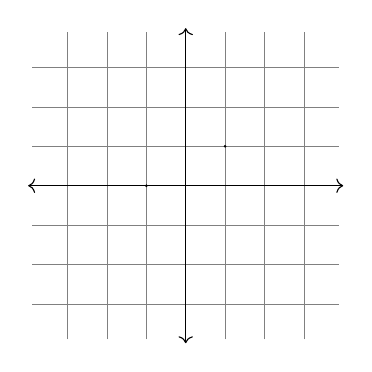
\begin{tikzpicture}[scale=.5]
            \draw[step=1,gray,very thin] (-3.9, -3.9) grid (3.9,3.9);
            \draw[<->] (-4, 0) -- (4, 0);
            \draw[<->] (0, -4) -- (0, 4);    
            \draw[fill] (1, 1) circle [radius=.5pt];
            \draw[fill] (-1, 0) circle [radius=.5pt];
        \end{tikzpicture}
        \end{center}
        % TODO : Question this is wrong ask why
        \item We know that the convec linear combinations of $P$ look like 
            \[
                \left\{ \vec{x} \in \mathbb{R}^2: \vec{x} = t\vec{e_1} + \left( 1 - t \right)\vec{e_2} = \mat{ t \\ \left( 1 - t \right) } \text{ for some  }t \in \left[ 0,1 \right]\right\}
            \]
            And so vectors in the range of $\mathcal{M}$ should be the set
            \[
                \left\{ \vec{x} \in \mathbb{R}^2: \vec{x} = \mat{ 1 & -1 \\ 1 & 0 }\mat{ t \\ \left( 1 - t \right)}  \right\}
            \]
            which are the vectors
            \[
                \mat{ 2t - 1 \\ t } = \left( 2t - 1 \right)\vec{e_1} + t\vec{e_2} \text{ for some  } t \in \left[ 0,1 \right]
            \]
            \begin{center}
                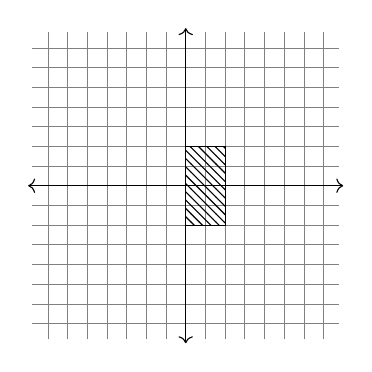
\begin{tikzpicture}[scale=0.5]
                    \draw[step=.5,gray,very thin] (-3.9, -3.9) grid (3.9, 3.9);
                    \draw[<->] (-4, 0) -- (4, 0);
                    \draw[<->] (0, -4) -- (0, 4);
                    \draw[pattern=north west lines] (0,-1) rectangle (1,1);
                \end{tikzpicture}
            \end{center}
            We know that the span of a vector in $X$ will look like $\mat{ \alpha \\ 0 }\text{ for some  } \alpha \in \mathbb{R}$ and so the range will end up looking like
        \[
        \left\{ \vec{x} \in \mathbb{R} : \vec{x}  = \mat{ 1 & -1 \\ 1 & 0 } \mat{ \alpha  \\ 0 } \right\} 
        \]
        And equivalently 
        \[
        \left\{ \vec{x} \in \mathbb{R} :\vec{x} = \mat{ \alpha  \\ \alpha  } \right\} 
        \]
        which is exactly $\mathit{span} {\left\{ \mat{ 1 \\ 1 } \right\} } $ 
        Drawing this we have
        \begin{center}
            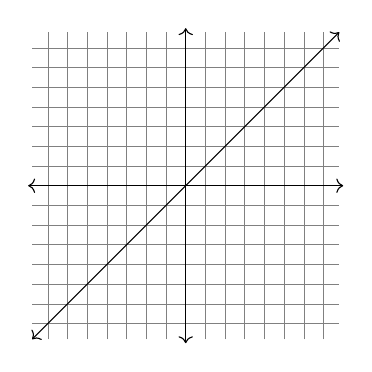
\begin{tikzpicture}[scale=0.5]
                \draw[step=.5,gray,very thin] (-3.9, -3.9) grid (3.9, 3.9);
                \draw[<->] (-4, 0) -- (4, 0);
                \draw[<->] (0, -4) -- (0, 4);
                \draw[<->] (-3.9, -3.9) -- (3.9,3.9);
            \end{tikzpicture}
        \end{center}
    \end{enumerate}
\item Let $\ell = \left\{ a \vec{v} \text{ for some  } a \in \left[ 0, \beta  \right] \text{ for some  } \beta \in \mathbb{R}   \right\} $ then we'll look at the image of $\mathcal{M} $ which will look like 
    \[
    \left\{ \vec{x} \in \mathbb{R}^2 : \vec{x} = \mat{ 1 & -1 \\ 1 & 0 } \alpha \mat{ x \\ y } \right\} 
    \]
    Which equivalenlty is 
    \[
        \left\{ \vec{x} \in \mathbb{R}^2 :\vec{x} = \mat{ \alpha x - \alpha y  \\ \alpha x  } \right\} 
    \]
    which gives us the vectors
    \[
    \alpha \mat{ x - y \\ x }
    \]
    Which by definition is a line segment.\\
    Alternatively we know that a line segment looks like $\alpha v + \vec{u} $ and that the image of this under some linear transformation $\mathcal{J} $ is the set of vectors $\left\{ \mathcal{J}\left(\alpha \vec{v}  + \vec{u} \right)  \right\}= \left\{ \alpha \mathcal{J}\left(\vec{v}\right)  + \mathcal{J}\left(\vec{u} \right)   \right\} $ which is also a line segment.
    \item Q3
    \begin{enumerate}
        \item $\mathcal{A}\left(\mathbb{R}^2 \right) $ is the set
            \begin{gather*}
                \left\{ \vec{v} \in \mathbb{R}^2 :\vec{v} = \mat{ x - 2y \\ -2x + 4y + 2 } \text{ for some  } \mat{ x \\ y } \in \mathbb{R}^2  \right\} 
            \end{gather*}
        \item $\mathcal{A}\left(B\right) $ is the set
            \begin{gather*}
                \left\{ \vec{v} \in \mathbb{R}^2 :\vec{v} = \mat{ x - 2y \\ -2x + 4y + 2 } \text{ for some  } \mat{ x \\ y } \in B  \right\} 
            \end{gather*}
    \end{enumerate}
    \item Q4
    \begin{enumerate}
        \item We know that the the xaxis is defined by the set $X$ 
            \[
            \left\{ \vec{x} \in \mathbb{R}^2 :\vec{x} = \mat{ \alpha  \\ 0 } \text{ for some  } \alpha \in \mathbb{R}  \right\} 
            \]
            And so the image under $\mathcal{Q} $ is the set 
            \begin{gather*}
                \left\{ \vec{v} \in \mathbb{R}^2 :\vec{v} = \mat{ x \\ y^2  } \text{ for some  } \mat{ x \\ y } \in X \right\} 
            \end{gather*}
            But we know the $y$ of any vector in $X$ is 0 so this just redfines the $X$ axis and we know that $\mathbb{R} $ is closed under addition and multiplication so this is certianly a subspace and a subset of $\mathbb{R}^2 $ for example take an element in $X$ and it's guarnteed to look like $\mat{ \alpha  \\ 0 } \subseteq \mathbb{R}^2 $ as required.
        \item Let's call the line segment $\ell $ and we know that the image of $\ell $ under $\mathcal{Q} $ is the set
            \[
                \left\{ \vec{v} \in \mathbb{R}^2 :\vec{v} = \mat{ 3t \\ \left( 2 + t \right) ^2  } \text{ for some  } t \in \left[ 0,1 \right]  \right\} 
            \]
            We know that $\left( 2 + t \right) ^2 = 4 + 4t + t^2  $ and so the vectors in the image are of the form
            \[
            \mat{ 0 \\ 4 }  + t \mat{ 3 \\ 4 + t } 
            \]
            Which defines a line that has been shifted, nevertheless it ends as $t \in \left[ 0,1 \right] $ and thus it is a segment as required.
    \end{enumerate}
    \item A line segment is a line that is described by $\alpha \vec{v} \text{ for some  } a \in \left[ 0, \beta  \right] \text{ for some  } \beta \in \mathbb{R} $ we know if we look at $\ell= \left\{ \alpha \vec{v} \text{ for some  } \alpha \in \mathbb{R}   \right\} $ where $\vec{v} \neq \vec{0} $ and $\vec{v} \neq \vec{\vec{e_1} } $ and $\vec{v} \neq \vec{e_2} $ that the image will result in a vshape which cannot be described as a single line segment
    \item Q5
    \begin{enumerate}
        \item 
            \begin{gather*}
                \left\{ \vec{v} \in \mathbb{R}^2 : \vec{v} = \mat{ e^{y} \cos{x} \\ e^{y} \sin{x} } \text{ for some  } \mat{ x \\ y } \in \mathbb{R}^2   \right\} \\
            \end{gather*}
    \end{enumerate}
\end{enumerate}

% subsection extra_handout (end)

% chapter week_9 (end)

\chapter{Week 10}%
\label{chp:week_10}
% chapter week_10

\section{Lecture 1}%
\label{sec:lecture_1}
% section lecture_1

Null space \& Range

\begin{defn}[Induced Transformation]\index{Induced Transformation}\label{defn:induced_transformation}
    Let $M$ be an $n \times m $ matrix. We say $M$ \hlnotea{induces} a linear transformation $T_{M} : \mathbb{R}^{m} \to \mathbb{R}^{M}$ defined by
    \begin{equation*}
        \left[ T_{M}\vec{v} \right]_{\mathcal{E'}} = M\left[ \vec{v} \right]_{\mathcal{E}}  
    \end{equation*}
    Notice that $\mathcal{E'} \text{ and } \mathcal{E} $ are standard basis
\end{defn}

\begin{eg}
    For example from the above definition if we have the vector $\vec{v} = \left[ \mat{ 1 \\ 2 } \right]_{\mathcal{B}}$ and we wanted to determine what $T_{M}\left(\vec{v}\right)$ is we must first translate $\left[ \mat{ 1 \\ 2 } \right]_{\mathcal{B}}$ to the standard basis. One method to do so is to find the matrix $X$ that translates from one basis to another. Then plug that new box of numbers into $M \left[ \vec{v} \right]_{\mathcal{E}}$ and we get our solution to $T_{M}\left(\vec{v}\right)$ 
\end{eg}

\begin{eg}
    The difference between $M\vec{v}$ and $M \left[ \vec{v} \right]_{\mathcal{E}}$ is the level of rigor? on the right we have something precise but on the left we don't. Also we can remember that $\left[ \vec{v} \right]_{\mathcal{E}}$ represents a box of numbers, the coordinates in the basis, where as $\vec{v}$ is assumed to be in the $\mathcal{E}$ basis but this could alos mean a vector just floating in space without any type of basis involved.
\end{eg}

\begin{eg}
    To determine what $\left[ T_{M}\vec{e_1} \right]_{\mathcal{E'}}$ use the fact that it's equal to $M\left[ \vec{e_1} \right]_{\mathcal{E}}$ and we know that this corresponds to the first column in $M$ as $\left[ \vec{e_1} \right]_{\mathcal{E}} = \mat{ 1 \\ 0 }$ 
\end{eg}

\begin{eg}
    We start by knowing that each column must be in the range of $T_{M}$ by inputting $\vec{e_i}$ into the equation. But we showed last time that the range is a subspace which means that if we find two elements in it, we know the sum and product of the vectors is also in the range, so we know that the span of each column is a susbset of the range. % TODO: why is this a susbset but not equal?
    We then want to see if the span of the columns is actually eqaual to the range, so we must show the other direction now. So let $\vec{x_{1}}, \vec{x_2} \in \mathit{range} {\left( T_{M} \right)} $ so we know that $\vec{x} = T_{M}\left(\vec{v}\right)$ for some $\vec{v} \in \mathbb{R}^{m} \Leftrightarrow \left[ \vec{x} \right]_{\mathcal{E'}} = \left[ T_{M}\left(\vec{v}\right) \right]_{\mathcal{E'}} \Leftrightarrow \left[ \vec{x} \right]_{\mathcal{E'}} = M \left[ \vec{v} \right]_{\mathcal{E}}$ and we recall that $M$ is only a list of vectors and that $\left[ \vec{v} \right]_{\mathcal{E}}$ is but a box of numbers and so using matrix vector multiplication we know that we just get a linear combination of the vectors as columns in $M$ and so we showed that $\vec{x}$ looks like a vector in the span of the columns of $M$ as we wanted.
\end{eg}

\begin{defn}[Fundamental Subspaces]\index{Fundamental Subspaces}\label{defn:fundamental_subspaces}
    Associated with any matrix $M$ are three fundamental subspaces: the \hlnotea{row space} of $M$,  denoted $row(M)$, is the span of the rows of $M$ the \hlnotea{column space} of M, denoted $col(M)$ , is the span of the columns of $M$; and the \hlnotea{null space} of $M$, denoted $\mathit{null} {\left( M \right)} $,  is the set of solutions to $M\vec{x} = 0$ 
\end{defn}

Let $A = \mat{ 1 & 0 & 0 \\ 0 & 1 & 0 }$ 

\begin{eg}
    We know that the row space is $\mathit{span} {\left\{ \mat{ 1 \\ 0 \\ 0 }, \mat{ 0 \\ 1 \\ 0 } \right\}} $ or
    
    $\left\{ \mat{ \alpha \\ \beta \\ 0 } \in \mathbb{R}^3, \text{ for some } \alpha, \beta \in \mathbb{R} \right\}$  
\end{eg}

\begin{eg}
    The column space of $A$ is $\mathit{span} {\left\{ \mat{ 1 \\ 0 }, \mat{ 0 \\ 1 }, \mat{ 0 \\ 0 } \right\}} $ or equivalently $\mathbb{R}^2$, we can tell instantly that the column space is not the same as the row space as one is in $\mathbb{R}^{3}$ where the othe is $\mathbb{R}^2$. 
\end{eg}

\begin{eg}
    We are looking for all the vectors that are perpendicular to $\mat{ 1 \\ 0 \\ 0 } \text{ and  } \mat{ 0 \\ 1 \\ 0 }$ so we require the the vectors $\vec{x} \in \mathbb{R}^3$ such that 
    \begin{gather*}
        \mat{ 1 \\ 0 \\ 0 } \cdot \mat{ x \\ y \\ z } = 0 \text{ and } \mat{ 0 \\ 1 \\ 0 } \cdot \mat{ x \\ y \\ z } = 0\\
        x + y = 0\\
        x = -y
    \end{gather*}
    And so we know all solutions are 
    \begin{equation*}
        \alpha \mat{ -1 \\ 1 \\ 0 } + \beta \mat{ 0 \\ 0 \\ 1 }, \text{ for all } \alpha, \beta \in \mathbb{R}
    \end{equation*}
\end{eg}

\begin{eg}
    For the null space of $A$ we know we are looking for all vectors $\mat{ x \\ y \\ z } \in \mathbb{R}^3$ so that
    \begin{gather*}
        A \mat{ x \\ y \\ z } = 0 \\
        \mat{ 1 & 0 & 0 \\ 0 & 1 & 0 } \mat{ x \\ y  \\ z } = 0\\
        \mat{ 1 \\ 0 }x  + \mat{ 0 \\ 1 }y   + \mat{ 0 \\ 0 }z   = \mat{ 0 \\ 0 }
    \end{gather*}
    So we determine that $x = y = 0$ but $z \in \mathbb{R}$ so we can think of this as the z axis coming out from the x y plane.
\end{eg}

\begin{eg}
    The range of $T_{A} : \mathbb{R}^3 \to \mathbb{R}^2 $ 
    \begin{gather*}
        \left\{ \vec{u} \in \mathbb{R}^2: T_{A}\left(\vec{x}\right) = \vec{u}, \text{ for some } \vec{x} \in \mathbb{R}^3 \right\} \\
        \left\{ \vec{u} \in \mathbb{R}^2: \mat{ 1 & 0 & 0 \\ 0 & 1 & 0 } = \vec{u}, \text{ for some } \vec{x} \in \mathbb{R}^3 \right\}
    \end{gather*}
    Which we know is saying that we are looking for the vectors $\vec{u}$  such that they are linear combinations of the columns of the matrix $A$ so equivalently we have that $\vec{u} \in \mathit{span} {\left\{ \vec{e_1}, \vec{e_2} \right\}} $ 

    We'll now look for the $\mathit{null} {\left( T_{A} \right)} $ we know that the nullspace is defined by 
    \begin{equation*}
        \left\{ \vec{x} \in \mathbb{R}^3 : T_{A}\left(\vec{x}\right) = 0 \right\}
    \end{equation*}
    So we're really looking for the vectors which satisfy $A \vec{x} = 0$, which is equivalent to $\mathit{null} {\left( A \right)} $ 
\end{eg}

Let $B = \mat{ 1 & 2 & 3 \\ 1 & 1 & 1 }$ $C = rref\left(B\right) = \mat{ 1 & 0 & -1 \\ 0 & 1 & 2 }$ 

\begin{eg}
    The row space of $B$ is equal to  $\mathit{span} {\left\{ \mat{ 1 \\ 2 \\ 3 }, \mat{ 1 \\ 1 \\ 1 } \right\}} $ and the row reducing involves the operations of addition and multiplication of the rows together, let $\vec{x}, \vec{u}$ represnt the first and second vectors in the span, we know that in the row reduced form (considering rows to be vectors) we have that the first row
    \begin{equation*}
        \mat{ 1 \\ 0 \\ -1 } = \vec{u} - \left( \vec{x} - \vec{u} \right)
    \end{equation*}
    and the second row
    \begin{equation*}
        \mat{ 0 \\ 1 \\ 2 } = \vec{x} - \vec{u}
    \end{equation*}
    Thus we know that the rows in the row reduced form are just linear combinations of the original rows, so we can say that
    \begin{equation*}
        row\left(B\right) = row\left(C\right)
    \end{equation*}
\end{eg}

\begin{eg}
    As for $\mathit{null} {\left( B \right)} = \left\{ \vec{x}: B \vec{x} = 0 \right\} $ the process of finding soltions to the zero vector will be identical to just row reducing, where it's an augmented matrix with 0's on the right side, so due to the same reasoning as before we know that they will have the same solutions as row operations don't change the number of solutions so we can say that 
    \begin{equation*}
        \mathit{null} {\left( B \right)}  = \mathit{null} {\left( C \right)} 
    \end{equation*}
\end{eg}

\begin{eg}
    Now if we are asked to compute the null space of $B$ then we can make things quite a bit easier on ourselves by using the row reduced matrix so well have
    \begin{gather*}
        \left\{ \vec{x} \in \mathbb{R}^3: B\vec{x} = 0 \right\}
    \end{gather*}
    So we're looking at the solutions to 
    \[
    \mat{ 1 & 0 & -1 \\ 0 & 1 & 2 } \mat{ x \\ y \\ z } = 0 
    \]
    Let $z = t$ for some $t \in \mathbb{R}$ then we determine $y = -2t$ and $x = t$ in general form we get
    \[
    t \mat{ 1 \\ -2 \\ 1 }, \text{ for all  } t \in \mathbb{R}
    \]
\end{eg}

Let $P = \mat{ 0 & 0 \\ 1 & 2 }$ and $Q = rref\left(P\right) = \mat{ 1 & 2 \\ 0 & 0 }$

\begin{eg}
    $col\left(P\right) = \mathit{span} {\left\{ \mat{ 0 \\ 1 }, \mat{ 0 \\ 2 } \right\}} = \mathit{span} {\left\{ \mat{ 0 \\ 1 } \right\}}$ and 
    $col\left(Q\right) = \mathit{span} {\left\{ \mat{ 1 \\ 0 } \right\}} $ We notice these are different so then row reduction can change the columns space unlike the row space.
\end{eg}

\begin{defn}[Rank]\index{Rank}\label{defn:rank}
    For a linear transformation $T : V \to W $,  the \hlnotea{rank} of $T$,  denoted $rank\left(T\right)$, is the dimension of the range of $T$ 

    For an $n \times m$ matrix $M$,  the \hlnotea{rank} of M, denoted $rank\left(M\right)$,  is the number of pivots in $rref\left(M\right)$ 
\end{defn}

Let $\mathcal{P}$ be the projection onto $\mathit{span} {\left\{ \vec{u} \right\}} $ where $\vec{u} = \mat{ 2 \\ 3 }$,  and let $\mathcal{R}$ be a rotation counter-clockwise by $\frac{\pi}{2}$ radians.

\begin{eg}
    $\mathit{range} {\left( \mathcal{P} \right)} $ is equal to $\mathit{span} {\vec{u}} $ because we know that every vector you choose will become some a scalar of $\mat{ 2 \\ 3 }$ thus the dimension is 1, so it's rank is 1.

    As for the rank of $\mathcal{R}$ we know that iwe we consider every vector in $\mathbb{R}^2$ and rotate them all $\frac{\pi}{2}$ radians then we still have all of $\mathbb{R}^2$ so we know that the rank is still 2.
\end{eg}

\begin{eg}
    We'll now find the rank of the matricies that go along with $\mathcal{P} \text{ and }\mathcal{R}$ first we know that the matricies are
    \begin{align*}
        \mathcal{P} = \frac{1}{13} \mat{ 4 & 6 \\ 6 & 9 } && \mathcal{R} = \mat{ 0 & -1 \\ 1 & 0 }
    \end{align*}
    Starting with $\mathcal{P}$ 
    \begin{gather*}
\begin{gmatrix}[b]
    4 & 6 \\
    6 & 9 
\end{gmatrix}
        \rightsquigarrow
\begin{gmatrix}[b]
    24 & 36 \\
    24 & 36 
\end{gmatrix}
        \rightsquigarrow
\begin{gmatrix}[b]
    24 & 36 \\
    0 & 0 
\end{gmatrix}
    \end{gather*}
    And so we know that there is one pivot so the rank of this matrix is 1

    As for $\mathcal{R}$ by swapping row one and row two we see that there must be two pivots and so the rank is 2.
\end{eg}


% section lecture_1 (end)

\section{Lecture 2}%
\label{sec:lecture_2}
% section lecture_2

Let $M$ be a matrix and recall that 
\begin{align*}
    row\left(M\right) = \mathit{span} {\text{ rows of M }}  && col\left(M\right) = \mathit{span} {\text{ cols of M }} 
\end{align*}

And that the following properties hold

\begin{align*}
    row\left(M\right) = row\left(rref\left(M\right)\right) && col\left(M\right) \neq col\left(rref\left(M\right)\right)
\end{align*}

Also we know that 
\begin{equation*}
    rank\left(M\right) = \text{ pivots of  } rref\left(M\right)
\end{equation*}

\begin{eg}
    If $M$ looked like this after row reduction we know it's rank is two (two pivots)
    \[
    \begin{gmatrix}[b]
    	a & b & c \\
    	d & e & f \\
    	j & i & k 
    \end{gmatrix}
    \rightsquigarrow
    \begin{gmatrix}[b]
    	1 & 0 & \alpha \\
    	0 & 1 & \beta \\
    	0 & 0 & 0 
    \end{gmatrix}
    \]
\end{eg}

\begin{crly}
    $\begin{WithArrows}
        rank\left(M\right) &= \text{ \# linearly independent columns of } rref\left(M\right)\\
        &= dim\left(col\left(rref\left(M\right)\right)\right) \Arrow{Solutions aren't lost}\\
        &= dim\left(col\left(M\right)\right) \\
        &= \text{ \# linearly independent columns of }M \\
        &= dim\left(row\left(rref\left(M\right)\right)\right) \Arrow{pivots are both \\horizontal and vertical} \\
        &= dim\left(row\left(M\right)\right) \\
    \end{WithArrows}$
\end{crly}

\begin{defn}[Transpose of a Matrix]\index{Transpose of a Matrix}\label{defn:transpose_of_a_matrix}
    The transpose of a matrix $M$ is the matrix $M^{T}$ whose rows are the columns of $M$ 
\end{defn}

\begin{eg}
    If 
    \[
    M = 
    \begin{bmatrix}
    	a & b \\
    	c & d 
    \end{bmatrix}
    \Leftrightarrow
    M^{T} = 
    \begin{bmatrix}
    	a & c \\
    	b & d 
    \end{bmatrix}
    \]
    Or 
    \[
    M = 
    \begin{bmatrix}
    	1 & 2 & 3 \\
    	4 & 5 & 6 
    \end{bmatrix}
    \Leftrightarrow
    M^{T} = 
    \begin{bmatrix}
    	1 & 4 \\
    	2 & 5 \\
    	3 & 6 
    \end{bmatrix}
    \]
\end{eg}

\begin{crly}
    \[
    rank\left(M\right) = rank\left(M^{T}\right)
    \]
    because $dim\left(col\left(M\right)\right) = dim\left(row\left(M\right)\right)$ and we know that $col\left(M\right) = row\left(M^{T}\right)$ 
\end{crly}

Find the rank of the following matricies
\begin{ex}
    $\mat{ 1 & 1 \\ 2 & 2 }$ we can see that there is one linearly independent vector so the dimension is 1 and rank is 1
\end{ex}

\begin{ex}
    $\mat{ 1 & 2 \\ 3 & 4 }$ we can see that there are 2 linearly independent vectors so dimension is 2 and rank is 2
\end{ex}

\begin{ex}
    $\mat{ 1 & 1 & 0 \\ 0 & 0 & 1 }$ We know that the dimension of the column space is 2 and thus rank is 2
\end{ex}

\begin{ex}
    $\mat{ 3 \\ 3 \\ 2 }$ the rank is 1, there is only one column
\end{ex}

Let $M$ be a $3 \times 4$ matrix whose rank is 3 does this mean that all of the columns of $M$ are linearly independent ?

No! if the matrix is $3 \times 4$ then we know that there are four columns, and if the rank is 3 we know 3 of the are linearly independent but we don't know about the last one, so we can't be sure.

What if $M$ was $4 \times 3$ then we could be sure that every column is linearly independent as we know that it must have 3 pivots and so it must be true.

\begin{thm}[Rank-nullity]\index{Rank-nullity}\label{thm:rank_nullity}
    The \hlnotea{nullity} of a matrix is the dimension of the null space.\\
    The rank-nullity theorem for a matrix $A$ states
    \[
    rank\left(A\right) + nullity\left(A\right) = \# \text{ of columns of  } A
    \]
\end{thm}

\begin{eg}
    If we have
    \begin{equation*}
        \begin{gmatrix}[b]
        	. & . & . & . & . \\
        	. & . & . & . & . \\
        	. & . & . & . & . 
        \end{gmatrix}
        \rightsquigarrow 
        \begin{gmatrix}[b]
        	1 & 0 & . & . & . \\
        	0 & 1 & . & . & . \\
        	0 & 0 & . & . & . 
        \end{gmatrix}
    \end{equation*}
    And let's assume that the last 3 columns are free variable columns so then we know that the solution to the zero vector will have three paramers $t_1, t_2, t_3 \in \mathbb{R}$ and so we know that the dimension of the nullspace will be 3 .
   % TODO : Question  Ask why this is true again. 
\end{eg}

\begin{eg}
    Let $\vec{u}, \vec{v} \in \mathbb{R}^{9}$ be linearly independent and $\vec{w} = 2\vec{u} - \vec{v}$ 
    \begin{equation*}
        A = 
        \begin{bmatrix}[c|c|c]
        	\vec{v} & \vec{u} & \vec{w} 
        \end{bmatrix}
    \end{equation*}
    We instantly know that the dimension of the column space of $A$ is 2 and so rank is 2 thus nullity is 1 by R-N-T

    As for $A^{T}$ we know that $A$ has two pivot columns and so $A^{T}$ also has 2, and so by R-N-T it has nullity of 7.
\end{eg}

\begin{thm}[Rank-nullity for linear transformations]\index{Rank-nullity for linear transformations}\label{thm:rank_nullity_for_linear_transformations}
    Let $T : V \to W $ be a linear transformation thus there is a matrix $A$ such that $T = T_{A}$ so 
    \begin{equation*}
        T\left(\vec{x}\right) = A\vec{x} \text{ for all } \vec{x}\in V
    \end{equation*}
    We know from \cref{thm:rank_nullity} that 
    \begin{align*}
        \text{ \# columns of  }A &= rank\left(A\right) + nullity\left(A\right) \\
                                 &= dim\left(col\left(A\right)\right) + dim\left(\mathit{null} {\left( A \right)} \right)\\
                                 &= dim\left( \mathit{range} {\left( T \right)}  \right) + dim\left( \mathit{null} {\left( T \right)}  \right) \\
    \end{align*}
    So we can finally say that 
    \begin{equation*}
        dim\left( \mathit{range} {\left( T \right)}  \right) + dim\left( \mathit{null} {\left( T \right)}  \right) = \text{ \# columns of }A
    \end{equation*}
\end{thm}

\subsection{Inverse Matrix}%
\label{sub:inverse_matrix}
% subsection inverse_matrix

\begin{defn}[Inverse Transformation]\index{Inverse Transformation}\label{defn:inverse_transformation}
    If it exsits, the inverse transformation of $T : R^{n} \to R^{m} $ is 
    \begin{equation*}
        T^{-1} : R^{m} \to R^{n} 
    \end{equation*}
    That satisfies the following properties 
    \begin{gather*}
        T\left(T^{-1}\left(\vec{x}\right)\right) = \vec{x} \text{ for all  } \vec{x} \in \mathbb{R}^{n}\\
        T^{-1}\left(T\left(\vec{y}\right)\right) = \vec{y} \text{ for all } \vec{y} \in \mathbb{R}^{m}
    \end{gather*}
    If $T = T_{A}$ and $T^{-1} = T_{B}$ then
    \begin{align*}
        \vec{x} &=  T\left(T^{-1}\left(\vec{x}\right)\right) \\
        &= T\left(B\vec{x}\right) \\
        &= AB\vec{x}
    \end{align*}
    But for this to be true for all $\vec{x} \in \mathbb{R}^{m}$ then we require
    \begin{equation*}
        AB = I
    \end{equation*}
    And if $A$  is $n \times m$ and $B$  is $m \times n$ then we know that $I$  is $n \times n$ \\
    Similarly $T^{-1}\left(T\left(\vec{y}\right)\right) = \vec{y} \Leftrightarrow BA = I$ \\
    Thus we say $B$ is the inverse Matirx of $A$ denoted $B = A^{}$ 
\end{defn}
\begin{defn}[Inverse Matrix]\index{Inverse Matrix}\label{defn:inverse_matrix}
    We say $B$  is the inverse matrix of $A$ denoted $B = A^{-1}$ if
    \begin{equation*}
        AB = BA = I
    \end{equation*}
\end{defn}

% subsection inverse_matrix (end)

% section lecture_2 (end)

\section{Tutorial 6}%
\label{sec:tutorial_6}
% section tutorial_6

\begin{enumerate}
    \item We say the function $T : \mathbb{R}^{n} \to \mathbb{R}^{m} $ is linear if we can say
    \begin{equation*}
        T\left(\vec{x} + \alpha\vec{y}\right) = T\left(\vec{x}\right) + \alpha T\left(\vec{y}\right) \text{ for all  } \vec{x}, \vec{y} \in \mathbb{R}n
    \end{equation*}
    \item
    \begin{enumerate}
        \item 
        \begin{proof}
            We'll show that $\mathcal{A}$ is linear so let $\vec{u}, \vec{v} \in \mathbb{R}^2$ and $\alpha \in \mathbb{R}$ we know that
            \begin{equation*}
                T\left(\vec{u} + \alpha \vec{v}\right) = T\left( \mat{ x_1 + \alpha x_2 \\ y1 + \alpha y_2 }\right) = \mat{ y_1 + \alpha y_2 \\ 0 \\ x_1 + \alpha x_2 } = T\left(\vec{u}\right) + \alpha T\left(\vec{v}\right)
            \end{equation*}
        \end{proof}
        \item We will show that $\mathcal{B}$ is not a linear transformation we know 
        \begin{equation*}
            \mathcal{B}\left(\mat{ -2 \\ 0 } + \mat{ 1 \\ 0 }\right) \neq \mathcal{B}\left(\mat{ -2 \\ 0 }\right) + \mathcal{B}\left(\mat{ 1 \\ 0 }\right)
        \end{equation*}
        \item We will show that $\mathcal{C}$ is a linear transformation it follows that 
        \begin{equation*}
            \mathcal{C}\left(\vec{u} + \alpha \vec{v}\right) = \vec{0} = \vec{0} + \alpha \vec{0} = \mathcal{C}\left(\vec{u}\right) + \alpha \mathcal{C}\left(\vec{v}\right)
        \end{equation*}
        \item We will show that $\mathcal{D}$ is not a linear transformation 
        \begin{equation*}
            \mathcal{D}\left(\vec{u} + \alpha \vec{v}\right) = \mat{ 1 \\ 1 } \neq \mat{ 1 \\ 1 } + \alpha \mat{ 1 \\ 1 } = \mathcal{D}\left(\vec{u}\right) + \alpha \mathcal{D}\left(\vec{u}\right)
        \end{equation*}
    \end{enumerate}
        \item We will now compute the null space, range and rank of each of the linear transformations
        \begin{enumerate}
            \item We'll start by comupting the range which we can we can say is
            \[
            \left\{ \vec{v} \in \mathbb{R}^3: \vec{v} = s \mat{ 1 \\ 0 \\ 0 } + t \mat{ 0 \\ 0 \\ 1 } \text{ for some } t, s \in \mathbb{R} \right\}
            \]
            we know that that null space is only $\vec{0}$, and that the rank must be 2 as a basis for the range is
            \[
            \left\{ \mat{ 1 \\ 0 \\ 0 }, \mat{ 0 \\ 0 \\ 1 } \right\}
            \]
            \item We'll start with the range
                % TODO : Question Is any of this right?
            \[
            \left\{ x \in \mathbb{R}: x \ge 0 \right\}
            \]
            And the null space is
            \[
            \left\{ x \in \mathbb{R}: x < 0 \right\}
            \]
            So then the rank of $\mathcal{B}$ is 0
            % TODO : Question Why?? 
            \item For $\mathcal{C}$ we know the range is
                \[
                \left\{ \vec{0} \right\}
                \]
                And then null space is 
                \[
                \left\{ \vec{x} \in \mathbb{R}^2 \right\}
                \]
                And then rank is 0
                % TODO : Question Why is it 0 shouldn't it be 1?
            \item The range of $\mathcal{D}$ is $\left\{ \mat{ 1 \\ 1 } \right\}$ and the null space is $\emptyset$ since $\mathcal{D}$ is not a subspace then there is no basis for it, so the rank doesn't exist.
        \end{enumerate}
        \item 
        \begin{enumerate}
            \item $\mathcal{X}$ : the tranformation invoked by the identity matrix.
            \item $\mathcal{Y}$ : cannot exist as we know $\mathit{range} {\left( Y \right)} \subseteq \mathbb{R}^2$ and so the dimension of $\mathcal{Y} \le 2$ 
            \item $\mathcal{Z}: \mathit{comp}_{\mat{ 1 \\ 1 \\ 1 }} {\vec{x}} $ which defines a line in 3d space thus has dimension 1 so rank is 1 
            \item $\mathcal{W}$: the identity transformation
            \item Impossible?
            % TODO : Question Ask bout this
        \end{enumerate}
\end{enumerate}


% section tutorial_6 (end)

\section{Extra Textbook Questions}%
\label{sec:extra_textbook_questions}
% section extra_textbook_questions

\begin{itemize}
    \item Q1
        \begin{enumerate}[label=\alph*)]
            \item We can see that $\mat{ 3 \\ 2 } $ and $\mat{ -4 \\ 5 } $ are linearly independent and so we know that we can use row operations to get this turn this matrix into the identity matrix.
            \begin{gather*}
                \begin{gmatrix}[b]
                	3 & -4 & 1 & 0 \\
                	2 & 5 & 0 & 1 
                    \rowops
                    \add[-1]{1}{0} 
                \end{gmatrix}
                \rightsquigarrow 
                \begin{gmatrix}[b]
                	1 & -9 & 1 & -1 \\
                	2 & 5 & 0 & 1 
                    \rowops
                    \add[-2]{0}{1} 
                \end{gmatrix}\\
                \rightsquigarrow 
                \begin{gmatrix}[b]
                	1 & -9 & 1 & -1 \\
                	0 & 23 & -2 & 3
                    \rowops
                    \mult{1}{\cdot \frac{1}{23}} 
                \end{gmatrix}
                \rightsquigarrow 
                \begin{gmatrix}[b]
                	1 & -9 & 1 & -1 \\
                	0 & 1 & -\frac{2}{23} & \frac{3}{23} 
                \end{gmatrix}\\
                \rightsquigarrow 
                \begin{gmatrix}[b]
                	1 & 0 & 1 - \frac{18}{23} & -1 + \frac{27}{23} \\
                	0 & 1 & -\frac{2}{23} & \frac{3}{23} 
                \end{gmatrix}
            \end{gather*}
            And so the inverse is 
            \[
            \frac{1}{23} \mat{ 5 & 4 \\ -2 & 3 }
            \]
            \item We can see that these are 3 linearly independent vectors and so it can be reduced to 3 pivots, so it is invertible
            \item We know that the third column is 2 of the first column plus the second column thus we know that after row reduction we will only get two pivots \todo{why again?} and thus we can't get the identity matrix as that is 3.  
            \item If we swap all the rows of this matrix and then reduce we can clearly see we can get the indentity matrix so we know it has an inverse
            \item Row reduce and see if it it has 4 pivots.
            \item Reduce upwards and we get the identity matrix, it's invertible.
        \end{enumerate}
    \item A2
        \begin{enumerate}[label=a)]
            \item Row reduce $B$ to I which we know must be possible as the columns are linearly independent and so $\vec{s} = B^{-1} \mat{ 1 \\ 1 \\ 1 }$ 
            \item $\vec{x} = B^{-1} \mat{ -1 \\ 0 \\ 1 }$ 
            \item Same as above.
        \end{enumerate}
    \item A4
        \begin{enumerate}[label=a)]
            \item If the rotation is counter clockwise by $\frac{\pi }{6}$ then then inverse must be a clockwise rotation by $\frac{\pi }{6}$.
            \item This subtracts 3 times the y component of the vector from the x component a given input vector, so to invert this we add 3 times the y component to the x component to cancel it back out, so the matrix that represents the operation is 
                \[
                \mat{ 1 & 3 \\ 0 & 1 }      
                \]
            \item This matrix represents multiplying the x component of the vector by 5, the inverse is multiplying the x component of the vector by $\frac{1}{5}$ which is represented by the matrix 
                \[
                \mat{ \frac{1}{5} & 0 \\ 0 & 1 } 
                \]
            \item For some vector in $ \vec{v} \in \mathbb{R}^3 $ we know that it looks like $\mat{ x \\ y \\ z } $, after being operated on by this matrix, we multiply $y$ by $-1$ and so we get $\mat{ x \\  - y  \\ z } $ so we have to multiply by the same matrix to get back so the inverse is 
                \[
                \mat{ 1 & 0 & 0 \\ 0 & -1 & 0 \\ 0 & 0 & 1 }
                \]
        \end{enumerate}
    \item A1
        \begin{gather*}
            \begin{gmatrix}[b]
            	1 & 0 & 0 \\
            	0 & 1 & 0 \\
            	0 & 0 & 1 
                \rowops
                \add[-5]{1}{0} 
            \end{gmatrix}
            \rightsquigarrow 
            \begin{gmatrix}[b]
            	1 & -5 & 0 \\
            	0 & 1 & 0 \\
            	0 & 0 & 1
                \rowops
                \swap{2}{1} 
            \end{gmatrix}\\
            \rightsquigarrow 
            \begin{gmatrix}[b]
            	1 & -5 & 0 \\
            	0 & 0 & 1 \\
            	0 & 1 & 0 
                \rowops
                \mult{1}{\cdot 6} 
                \mult{2}{\cdot -1} 
                \add[4]{0}{2} 
            \end{gmatrix}
            \rightsquigarrow 
            \begin{gmatrix}[b]
            	1 & -5 & 0 \\
            	0 & 0 & 6 \\
            	4 & -21 & 0 
            \end{gmatrix}
        \end{gather*}
        Thus we know 
        \[
            \mat{ 1 & 0 & 0 \\ 0 & 0 & 0 \\ 4 & 0 & 1 } \mat{ 1 & 0 & 0 \\ 0 & 6 & 0 \\ 0 & 0 & 1 } \mat{ 1 & 0 & 0 \\ 0 & 1 & 0 \\ 0 & 0 & -1 } \mat{ 1 & 0 & 0 \\ 0 & 0 & 1 \\ 0 & 1 & 0 } \mat{ 1 & -5 & 0 \\ 0 & 1 & 0 \\ 0 & 0 & 1 } = B
        \]
        Where $B$ is the matrix which does all the row operations at once.
    \item A3
        \begin{enumerate}[label=\alph*)]
            \item add $-4$ row 2 to row 3
            \item multiply row 1 and row 3 by $-1$ (not elementary)
            \item multiply row 1 by 3 and add row 3 (not elementary)
            \item swap row 1 and 3
            \item d) then swap row 1 and 2 (not elementary)
            \item do nothing \todo{is this elementary?} 
        \end{enumerate}
    \item A4
        \begin{enumerate}[label=\alph*)]
            \item We'll start by describing the elementary row operations to get to $A$ from $I$. 
                \begin{itemize}
                    \item swap row 2 and 3
                    \item add 3 row 3 to row 1
                    \item multipy row 2 by 2
                    \item add 2 row 2 to row 1
                \end{itemize}
            To undo this we do
                \begin{itemize}
                    \item add $-2$ row 2 to row 1
                    \item multiply row 2 by $\frac{1}{2}$ 
                    \item add $ - 3$ row 3 to row 1
                    \item swap row 2 and 3
                \end{itemize}
            These steps represented as a matrix look like
            \[
            \mat{ 1 & 0 & 0 \\ 0 & 0 & 1 \\ 0 & 1 & 0 }\mat{ 1 & 0 & -3 \\ 0 & 1 & 0 \\ 0 & 0 & 1 }\mat{ 1 & 0 & 0 \\ 0 & \frac{1}{2} & 0 \\ 0 & 0 & 1 }\mat{ 1 & -2 & 0 \\ 0 & 1 & 0 \\ 0 & 0 & 1 }
            \]
            Which is the matrix
            \begin{gather*}
                \begin{gmatrix}[b]
                	1 & 0 & 0 \\
                	0 & 1 & 0 \\
                	0 & 0 & 1
                    \rowops
                    \add[-2]{1}{0} 
                \end{gmatrix}
                \rightsquigarrow 
                \begin{gmatrix}[b]
                	1 & -2 & 0 \\
                	0 & 1 & 0 \\
                	0 & 0 & 1 
                    \rowops
                    \mult{1}{\cdot \frac{1}{2}} 
                    \add[-3]{2}{0} 
                    \swap{1}{2} 
                \end{gmatrix}
                \rightsquigarrow 
                \begin{gmatrix}[b]
                	1 & -2 & -3 \\
                	0 & 0 & 1 \\
                	0 & \frac{1}{2} & 0 
                \end{gmatrix}
            \end{gather*}
        A is the product of the inverse operations as matricies ofthe steps to get to I from A, we can use the list I provided earlier. The rest of the questions are the same.
        \end{enumerate}
\end{itemize}

% section extra_textbook_questions (end)

% chapter week_10 (end)

\chapter{Week 11}%
\label{chp:week_11}
% chapter week_11

\section{Inverses}%
\label{sec:inverses}
% section inverses

\subsection{56}%
\label{sub:56}
% subsection 56

We start by applying some row operations to some identity matrices
\begin{gather*}
    \begin{gmatrix}[b]
    	1 & 0 & 0 \\
    	0 & 1 & 0 \\
    	0 & 0 & 0
        \rowops
        \add[2]{0}{2} 
    \end{gmatrix}
    \rightsquigarrow 
    \begin{gmatrix}[b]
    	1 & 0 & 0 \\
    	0 & 1 & 0 \\
    	2 & 0 & 1 
    \end{gmatrix}= E_{1} \\
    \begin{gmatrix}[b]
    	1 & 0 & 0 \\
    	0 & 1 & 0 \\
    	0 & 0 & 1
        \rowops
        \add[-2]{0}{2} 
    \end{gmatrix}
    \begin{gmatrix}[b]
    	1 & 0 & 0 \\
    	0 & 1 & 0 \\
    	-2 & 0 & 1 
    \end{gmatrix} = E_{2} 
\end{gather*}

Applying $E_{1} \text{ and } E_2$ to $A$ we can see...
\begin{gather*}
    \begin{bmatrix}
    	1 & 2 & 3 \\
    	4 & 5 & 6 \\
    	7 & 8 & 9 
    \end{bmatrix}
    \begin{bmatrix}
    	1 & 0 & 0 \\
    	0 & 1 & 0 \\
    	2 & 0 & 1 
    \end{bmatrix}
    = 
    \begin{bmatrix}
    	1 & 2 & 3 \\
    	4 & 5 & 6 \\
    	2 \cdot 1 + 7 & 2 \cdot 2 + 8 & 2 \cdot 3 + 9 
    \end{bmatrix}
\end{gather*}


Which we note is the same thing as adding twice the first row to the third. Then we know that $E_2A$ would be subtracting two of row 1 from row 3.

If we apply $E_1$ then $E_2$ then we just added and subtraced the first row which does nothing so $E_1E_2 = I= E_2E_1$ 
    

% subsection 56 (end)

\subsection{57}%
\label{sub:57}
% subsection 57

We know that matrix $A$ represents adding twice row 2 to row1 and adding -3 row 1 to row 3, by observation these operations will turn $D$ into the identity matrix, now let's look at it the other way.\\
We can see that matrix $D$ represents adding 3 of row 1 to row 3 then adding -2 row 2 to row 1 which we can tell are the inverse operations as what $A$ does so we know this will yield the identity matrix. So we can say $A$ and $D$ are inverses of each other.



% subsection 57 (end)

We'll now prove why the algorithm to determine the inverse matrix actually works, for example if we have the matrix 
\[
\begin{bmatrix}
    1 & 4 \\
    0 & 2 
\end{bmatrix}
\]
Then we would set something up like this
\[
\begin{bmatrix}[cc|cc]
    1 & 4 & 1 & 0 \\
    0 & 2 & 0 & 1 
\end{bmatrix}
\]
Where on the right hand side we have the matrix that will hold an of the ro operations we do to transform this matrix on the left into the identity matrix, thus once we're done the matrix on the right will represent all the row operations that would tern it into the identity matrix.

So it's just a way of keeping track of two different pieces of data visually.

\begin{gather*}
    \intertext{multiply row 2 by $\frac{1}{2}$, so now the matrix on the right represents this operation}
    \begin{bmatrix}[c c | c c]
    	1 & 4 & 1 & 0 \\
    	0 & 1 & 0 & \frac{1}{2} 
    \end{bmatrix}\\
    \intertext{add -4 of row 2 to row 1}
    \begin{bmatrix}[c c | c c]
    	1 & 0 & 1 & -2 \\
    	0 & 1 & 0 & -\frac{1}{2} 
    \end{bmatrix}
\end{gather*}

And then we know the matrix on the right represents applying the two row operations that turn the matrix on the left into the identity matrix upon multiplication by the matrix. Thus we've found the inverse matrix for the left matrix.

\begin{thm}[Inverse Existance]\index{Inverse Existance}\label{thm:inverse_existance}
    A matrix has an inverse if and only if it is square and can be ``row reduced" to the identity matrix.\\
    % TODO : Question Ask why it must be square
    We know you can reach the identity matrix if you can reach row reduced echolelon form which means you must have a pivot for each column, so we also require that the columns must be linearly independent.
\end{thm}

\begin{remark}
    If it's not square it's not one to one and onto, you are losing a dimesion. \todo{What does this mean?} 
\end{remark}

\begin{remark}
    Equivalent to \cref{thm:inverse_existance} we can require the rows be linearly independent as we know that $\mathit{dim} \left(\mathit{row} \left(A\right) \right) = \mathit{dim} \left(\mathit{col} \left(A\right) \right)= \mathit{rank} \left(A\right)  $  \todo[inline]{Why do we know this again?} 
\end{remark}

\subsection{59}%
\label{sub:59}
% subsection 59

By definition $A^{-1} A = I$ and so since we know that $A$ has an inverse, then then we know there we know it must have been able to be reduced to the $I$ with row operations, thus $\mathit{rank} \left(A\right) = I$ 

\begin{eg}
    Let $C$ be the matrix whose left columns are $A$ and rightmost column is $\vec{b} $ we know that this represents the following 
    \[
    A \mat{ x \\ y \\ z } = \vec{b} 
    \]
    so then we can say that
    \[
    \mat{ x \\ y \\ z } = A^{-1} \vec{b} 
    \]
    by multiplying by the inverse of $A$ to both sides.
\end{eg}

% subsection 59 (end)

\subsection{60}%
\label{sub:60}
% subsection 60

We know that if we have two square matricies $X,Y$ that $\left( XY \right) ^{-1} $ is the matrix $A$ such that $A\left( XY \right) = I$ and we require that $\left( XY \right) A= I$ in this case we know we just need the inverses next to eachother and this will cause a chain reaction of identity matrices so we can see that $\left( XY \right) ^{-1} = Y^{-1} X^{-1} $ 

% subsection 60 (end)

\subsection{61}%
\label{sub:61}
% subsection 61

We know that $ \vec{e_1} = \frac{1}{2}\vec{b_1} + \frac{1}{2}\vec{b_2} $ and so $\left[ \vec{e_1}  \right]_{\mathcal{B}} = \mat{ \frac{1}{2} \\ \frac{1}{2} } $ and then $\vec{e_2} = \frac{1}{2}\vec{b_1}  - \frac{1}{2}\vec{b_2} $ so we know that $\left[ \vec{e_2}  \right]_{\mathcal{B}} = \mat{ \frac{1}{2} \\ -\frac{1}{2} } $. 

We know that $X= \mat{ \vec{b_1}  & \vec{b_2}  }$ let's assume we have a vector such that $\left[ v \right]_{\mathcal{B}} = \mat{ \alpha  \\ \beta  } $  so we know that $X$ converts to standard basis.
\begin{equation*}
    X\mat{ \alpha  \\ \beta  } = \alpha \vec{b_1}  + \beta \vec{b_2} = \left[ \vec{v}  \right]_{\mathcal{E}} 
\end{equation*}

And thus we know $X\left[ \vec{e_2}  \right]_{\mathcal{B}} = \left[ \vec{e_2}  \right]_{\mathcal{E}} = \mat{ 1 \\ 0 } $ and $X\left[ 31 \right]_{\mathcal{B}} = \left[ \vec{e_1}  \right]_{\mathcal{E}} = \mat{ 1 \\ 0 } $. 

% subsection 61 (end)

\subsection{62}%
\label{sub:62}
% subsection 62

\begin{itemize}
    \item We know that  $X^{-1} $ should exists since the vectors in $\mathcal{B} $ form a basis so each is linearly independent thus row reduction will lead to reduced row echelon form and since $X$ is square we know that $X^{-1} $ must exist. 
    \item We know that if $X$ is the matrix that converts from $\mathcal{B} $ to $\mathcal{E} $ and so $X^{-1} $ must convert $\mathcal{E} \to \mathcal{B}$ \todo{explain why this is true} 
        \[
        X^{-1} \left[ \vec{v}  \right]_{\mathcal{E}} = \left[ \vec{v}  \right]_{\mathcal{B}} 
        \]

\end{itemize}

% subsection 62 (end)

% section inverses (end)

\section{Lecture 2 Week 11}%
\label{sec:lecture_2_week_11}
% section lecture_2

Recall: we say $M$ induces the linear transformation 
\[
T : \mathbb{R} ^{n}  \to \mathbb{R} ^{n}  \tag{$\alpha $}
\]
Or $M$ is the matrix corresponding to $T$ if 
\[
\left[ T\left(\vec{v} \right) \right]_{\mathcal{E}} = M\left[ \vec{v}  \right]_{\mathcal{E}} 
\]
Where $\mathcal{E} $ is the standard basis for $\mathbb{R} ^{n} $ and $T_{M} = T$ \\
If we don't sepcify the basis, then $\mathcal{E} $ is assumed. So we can replace $\alpha $  by $T\left(\vec{v} \right)= M\vec{v} $ 


Some properties follow
\begin{enumerate}
    \item We say $T_{M} $ and $T_{N} $ are inverses $\Leftrightarrow$ $M$ and $N$ are inverses \todo[color=green!40]{Prove this!} 
    \item $T_{M} $ is invertible $\Leftrightarrow$ $M$ is invertaible in which case
        \[
            \left( T_{M}  \right) ^{-1} = T_{M^{-1} } 
        \]
    \item We define the folowing notation 
        \[
        M= \left[ T \right]_{\mathcal{E}} 
        \]
        Means that $M$ is the matrix for $T$ in the $\mathcal{E} $ basis such that $\alpha $  holds
    \item If $\mathcal{B} $ is a nother basis for $\mathbb{R} ^{n} $ and $A= \left[ T \right]_{\mathcal{B}} $ then $A$ is the matrix for $T$ in the basis $\mathcal{B} $ so we know 
        \begin{equation*}
            \left[ T\left(\vec{v} \right) \right]_{\mathcal{B}} = A\left[ \vec{v}  \right]_{\mathcal{B}} \text{ for all  } \vec{v} \in \mathbb{R} ^{n} 
        \end{equation*}
\end{enumerate}

\begin{eg}
    Let $n= 2$ $\mathcal{B} = \left\{ \vec{b_1} , \vec{b_2}  \right\} $ and $\left[ \vec{b_1}  \right]_{\mathcal{E}} $ and $\left[ \vec{b_2}  \right]_{\mathcal{E}} = \mat{ 0 \\ 1 } $ so this means
    \begin{align*}
        \vec{b_1} = 1\vec{e_1}  + 1\vec{e_2}  && \vec{b_2} = 0\vec{e_1} 1 + 1\vec{e_2} 2
    \end{align*}
    And sayign $b_1= \left[ \mat{ 1 \\ 1 }  \right]_{\mathcal{E}} $ is the vector whose $\mathcal{E} $ coordinaqtes are $\mat{ 1 \\ 1 } $ and similarly $b_2$ coordinates are $\mat{ 0 \\ 1 } $ when we are looking at the $\mathcal{E} $ basis. 
\end{eg}

\begin{eg}
    If $\left[ T \right]_{\mathcal{B}} = \mat{ 1 & 2 \\ 3 & 4 }$ then we can say 
    \begin{equation*}
        T\left(\left[ \mat{ 1 \\ 1 }  \right]_{\mathcal{E}} \right)= T\left(\vec{b1} \right)= T\left(\left[ \mat{ 1 \\ 0 }  \right]_{\mathcal{}} \right)
    \end{equation*}
    Remember here that $\left[ \mat{ 1 \\ 1 }  \right]_{\mathcal{E}} $ is the vector in $\mathcal{E} $ cordinates 
    And the result of this will be 
    \[
    \left[ A \mat{ 1 \\ 0 }  \right]_{\mathcal{B}} = \mat{ 1 \\ 3 } _{B} = \vec{b_1}  + 3\vec{b_2} = \mat{ 1 \\ 4 } _{\mathcal{E} } 
    \]
\end{eg}

\begin{remark}
    say we have $\left[ \vec{v}  \right]_{\mathcal{E}} $ and we are trying to find what is $\left[ T\left(\vec{v} \right) \right]_{\mathcal{E}} $ and all we know is $A$ which is the matrix which which induces the transformation $T$ for vectors written in the $\mathcal{B} $ basis, then the process could look like this.
    \[
    \left[ \vec{v}  \right]_{\mathcal{E}} \implies \left[ \vec{v}  \right]_{\mathcal{B}} \implies A\left[ \vec{v}  \right]_{\mathcal{B}} =  \left[ T\left(\vec{v} \right) \right]_{\mathcal{B}} \implies \text{ convert to $\mathcal{E} $  } \implies \left[ T\left(\vec{v} \right) \right]_{\mathcal{E}} 
    \]
\end{remark}

\begin{remark}
    There has recently been a source of confusion relating to change of basis, so here is what you have to remember.
    \begin{gather*}
        \left[ \vec{v}  \right]_{\mathcal{B}} =  \mat{ \alpha  \\ \beta  } \tag{a box of numbers}\\
        \left[ \mat{ \alpha  \\ \beta  }  \right]_{\mathcal{B}} =  \alpha \vec{b_1}  + \beta \vec{b_2} =  \vec{v} 
    \end{gather*}
\end{remark}

\begin{eg}
    Alternatively if our goal was to find $\left[ T\left(\vec{b_1} \right) \right]_{\mathcal{E}} $ then we could have done this.
    \begin{align*}
        \left[ T\left(\vec{b_1} \right) \right]_{\mathcal{B}} &=  A\left[ \vec{b_1}  \right]_{\mathcal{B}} \\  
        &= A \mat{ 1 \\ 0 }  \\
        &= \mat{ 1 \\ 3 } \tag{a box of numbers for the $\mathcal{B}$ basis}
    \end{align*}
    So then we know that 
    \[
    T\left(\vec{b_1} \right)=  \vec{b_1}  + 3\vec{b_2} =  \mat{ 1 \\ 4 } _{\mathcal{E} } 
    \]
\end{eg}

\subsection{63}%
\label{sub:63}
% subsection 63

\begin{itemize}
    \item We know by definition that $\left[ \vec{c_1}  \right]_{\mathcal{C}} =  \mat{ 1 \\ 0 } \text{ and } \left[ \vec{c_2}  \right]_{\mathcal{C}} =  \mat{ 0 \\ 1 } $ 
    \item we know the following is true
        \begin{align*}
            T\left(\mat{ 2 \\ 1 } _{\mathcal{E} } \right)=  T\left(\vec{c_1} \right)=  2\vec{c_1}  && T\left(\mat{ 5 \\ 3 } _{\mathcal{E} } \right)=  T\left(\vec{c_2} \right)=  \vec{c_2} 
        \end{align*}
    \item We already know that $T\vec{c_1} =  2\vec{c_1} \text{ and } T\vec{c_2} =  \vec{c_2}  $ so then we know
        \begin{align*}
            \left[ 2\vec{c_1}  \right]_{\mathcal{C}} =  \mat{ 2 \\ 0 }  && \left[ \vec{c_2}  \right]_{\mathcal{C}} =  \mat{ 0 \\ 1 } 
        \end{align*}
    \item We know that $\mat{ \alpha  \\ \beta  } _{\mathcal{C} } =  \alpha \vec{c_1}  + \beta \vec{c_2} $ so then
        \begin{equation*}
            T\left(\alpha \vec{c_1}  + \beta \vec{c_2} \right)=  \alpha T\left(\vec{c_1} \right) + \beta T\left(\vec{\vec{c_2} } \right)=  \alpha 2\vec{c_1}  + \beta \vec{c_2} =  \mat{ 2\alpha  \\ \beta  }   
        \end{equation*}
    \item Let $X$ be the matrix which induces the transformation $T$ on elements of the $\mathcal{C} $ basis we know the following
        \[
        \left[ T\left(\vec{c_1} \right) \right]_{\mathcal{C}} =  X\left[ \vec{c_1}  \right]_{\mathcal{C}} 
        \]
        But we have $\left[ T\left(\vec{c_1} \right) \right]_{\mathcal{C}} =  \mat{ 2 \\ 0 } $ we also know that $\left[ T\left(\vec{c_2} \right) \right]_{\mathcal{C}} =  \mat{ 0 \\ 1 } $ and thus 
        \[
        X=  \mat{ 2 & 0 \\ 0 & 1 }
        \]
        And here we know that $X =  \left[ T \right]_{\mathcal{C}} $ 
    \item We know that we want to find $\left[ T \right]_{\mathcal{E}} $, remember that's the matrix $K$ such that the following properties holds 
        \[
        \left[ T\left(\vec{v} \right) \right]_{\mathcal{E}} = K\left[ \vec{v}  \right]_{\mathcal{E}} 
        \]
        Here's the plan, we know letting $\vec{v} = \vec{e_1} \text{ or } \vec{e_2} $ will give us the columns of $K$ but we must determine what $T\left(\vec{v} \right)$ is then convert that into the $\mathcal{E} $ basis. Though know what $\left[ T \right]_{\mathcal{C}} $ is which is useful in the following formula
        \begin{equation*}
            \left[ T\left(\vec{v} \right) \right]_{\mathcal{C}} = \left[ T \right]_{\mathcal{C}} \left[ \vec{v}  \right]_{\mathcal{C}} 
        \end{equation*}
    Ok, so let's start by converting $\vec{e_1} $ to the other basis, by observation we can tell that $\vec{e_1} = 3\vec{c_1}  - \vec{c_2} \Leftrightarrow \left[ \vec{e_1}  \right]_{\mathcal{C}} = \mat{ 3 \\ -1 } $ and also that $\vec{e_2} = -5\vec{c_1}  + 2\vec{c_2} \Leftrightarrow \left[ \vec{e_2}  \right]_{\mathcal{C}} = \mat{ -5 \\ 2 } $ and now we know 
    \begin{align*}
        \left[ T\left(\vec{e_1} \right) \right]_{\mathcal{C}} &= \mat{ 2 & 0 \\ 0 & 1 }\mat{ -5 \\ 2 }  \\
        &= \mat{ -10 \\ 2 }
    \end{align*}
    And also 
    \begin{align*}
        \left[ T\left(\vec{e_2} \right) \right]_{\mathcal{C}} &= \mat{ 2 & 0 \\ 0 & 1 } \mat{ 3 \\ -1 } \\
        &= \mat{ 6 \\ -1 }
    \end{align*}
    And thus we know that $T\left(\vec{e_2} \right)= \mat{ 7 \\ 3 } _{\mathcal{E} } $ and $T\left(\vec{e_1} \right) = \mat{ -10 \\ -4 } _{\mathcal{E} } $ and thus 
    \[
    K= \mat{ -10 & 7 \\ -4 & 3 }
    \]
    Alternatively we already know that $A^{-1} $ columns are $\left[ \vec{e_1}  \right]_{\mathcal{C}} \text{ and } \left[ \vec{e_2}  \right]_{\mathcal{C}} $ so we could have gone from there then multiplied by $\left[ T \right]_{\mathcal{C}} $ to get what $T\left(\vec{c_1} \right) \text{ and } T\left(\vec{c_2} \right)$ were.
\end{itemize}

% subsection 63 (end)

\section*{Tutorial 7}%
\label{sec:tutorial_7}
% section tutorial_7

\begin{itemize}
    \item Q1
        \begin{itemize}
            \item If $f$ is invertible this means that there exists a function $f^{-1} $ such that 
            \begin{gather*}
                f \circ f^{-1} = I\\
                f^{-1}  \circ f = I\\
                f\left(f^{-1} \left(\vec{x} \right)\right)= \vec{x} \text{ for all  } \vec{x} \text{ in f's range } \\
                f^{-1} \left(f\left(\vec{x} \right)\right)= \vec{x} \text{ for all  } \vec{x} \text{ in f's domain }\\
            \end{gather*}
            \item We say that $A$ is invertible if there exists a matrix $A^{-1} $ such that 
            \begin{equation*}
                A A^{-1} = I= A^{-1} A
            \end{equation*}
        \end{itemize}
    \item Q2
        \begin{itemize}
            \item We know that a is incorrect since matrix multiplication isn't commutative that is for any two matricies $A, B$ 
            \begin{equation*}
                AB \neq BA      
            \end{equation*}
            \item b is correct they multiplied by $A^{-1} $ from the left to both right hand side and left hand side .
            \item This is incorrect division by a matrix is not defined $\frac{1}{A}$ 
            \item d also fails due to the same reason as c.
            \item division is not defined for vectors and so $\frac{1}{\vec{b} }$ doesn't make sense.
        \end{itemize}
    \item Q3
        \begin{itemize}
            \item R
                \begin{itemize}
                    \item We know it is invertible as the inverse function exists, namely the transformation $R^{-1} $, a rotation counter clockwise by $\frac{\pi }{6}$ 
                    \item If we imagine all vectors in $\mathbb{R}^2 $ that have undergone a rotation of $\frac{\pi }{6} $ we still have $\mathbb{R}^2 $ and thus $\mathit{rank} \left(R\right) = 2$ 
                \end{itemize}
            \item D
                \begin{itemize}
                    \item We know that it is invertible as the inverse transformation exists namely anothether reflection about the line $y= 4x$ 
                    \item If we imagine the image of $\mathbb{R}^2 $ under $D$ we can see that everything above and below the line get swapped, this still spans all of $\mathbb{R}^2 $ and so the $\mathit{rank} \left(R\right) = 2$ 
                \end{itemize}
            \item P
                \begin{itemize}
                    \item We know that $P$ does not have an inverse, for example multiples of a normal vector for the line $y= 4x$ will all get mapped to the zero vector thus the $P^{-1} \left(\vec{0}\right)$ doesn't have a unique value associated with it. 
                    \item We know that the range looks like scalar multiples of the vector $\mat{ 1 \\ 4 } $ thus a basis is the set $\left\{ \mat{ 1 \\ 4 }  \right\} $ and so $\mathit{rank} \left(  P\right) = 1 $ 
                \end{itemize}
            \item S
                \item We know that $S$ is invertible as there exists $S^{-1} $ namely halving the length of every vector.
                \item Doubling every vector still will span $\mathbb{R}^2 $ and thus we know $\mathit{rank} \left(S\right) = 2$  
        \end{itemize}
    \item Q4
        \begin{itemize}
            \item I believe that a transformation $T : V \to W $   has an inverse if and only if $\mathit{rank} \left(V\right) = \mathit{rank} \left(W\right) $ 
            \begin{proof}
                For contradiction let's assume that $T$ has an inverse but $\mathit{rank} \left(V\right) \neq \mathit{rank} \left(W\right) $ . Let $n= \mathit{rank} \left(V\right) \text{ and } k= \mathit{rank} \left(W\right) $ 
                \begin{itemize}
                    \item Case 1 $n < k$ 
                        \begin{itemize}
                            \item We know that a basis for $V$ has n elements
                            \[
                            \left\{ \vec{v_1} , \ldots, \vec{v }_{n}   \right\} 
                            \]
                            
                                and thus the range of $T$ looks like $\left\{ \vec{x} \in W: \vec{x} = T\left(\vec{y}\right) \text{ for some  } y \in V  \right\} $ and thus the range is 
                                \[
                                \left\{ T\left(\alpha _{1} \vec{v_1} + \dotsb  + \alpha _{5} \vec{v_5} \right) \text{ for some  } \alpha_{1} ,\ldots,\alpha _{n} \in \mathbb{R}  \right\} 
                                \]
                                which will be 
                                \[
                                \mathit{span} {T\left(\vec{v_1} \right), \ldots, T\left(\vec{v}_{n}  \right)} 
                                \]
                                and so the dimension of the range is less than or equal to $n$ so there will be vectors in $W$ that are not reached as it's dimension is greater than $n$ and so the inverse of these vectors won't be defined, so the inverse must not exist which is a contradiction.
                        \end{itemize}
                    \item Case $n > k$.
                        \begin{itemize}
                            \item Making the same argument as above shows but looking at the range of $T^{-1} $ will give the same contradiction.
                        \end{itemize}
                \end{itemize}
            \end{proof}
        \end{itemize}
    \item We will determine the matrix which rotates a vector by $\theta $. We know that when $\vec{e_1} $ is rotated by $\theta $ that this situation is the same as the unit circle, in which we determined the $x,y$ coordinates to be $\cos{\theta}, \sin{\theta}  $ respectively as the hypotenuse is 1, thus we know that the first row of the matrix we are looking for is $\mat{ \cos{\theta}  \\ \sin{\theta}     }$. We'll determine the second row now by seeing what happens to $\vec{e_2} $ which gives the angle $\frac{\pi }{2} + \theta $ we know that sine of this angle is still the same thing but cosine of this angle is $ - \cos{\theta} $ and so the generic rotation matrix of $\theta $ radians is given by
        \[
            \mat{ \cos{\theta}  &  - \sin{\theta}  \\ \sin{\theta}  & \cos{\theta}  }
        \]
    \item We'll now observer what happens when $\vec{e_1} $ and $\vec{e_2}$ are reflected across the line $y = mx$ for some $m \in \mathbb{R}$ 
        \begin{center}
            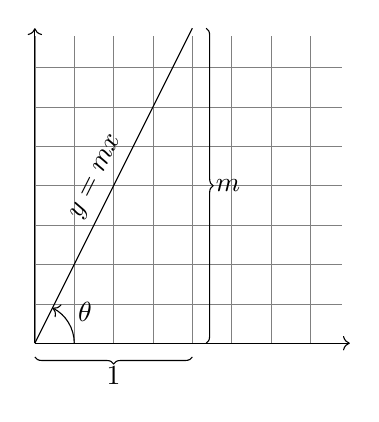
\begin{tikzpicture}
                \draw[step=.5,gray,very thin] (0,0) grid (4.0 - 0.1, 4.0 - 0.1);
                \draw[->] (0, 0) -- (4.0, 0);
                \draw[->] (0, 0) -- (0, 4.0);
                \draw[-] (0,0) -- (2, 4) node[midway, above, sloped]{$y=mx$ } ;
                \coordinate (c) at (2, 4);
                \coordinate (b) at (0,0);
                \coordinate (a) at (2, 0);
                \pic [draw, ->, "$\theta$", angle eccentricity=1.5] {angle = a--b--c};
                \draw[decoration={brace,mirror,raise=5pt},decorate] (0, 0) -- node[midway, below, yshift=-5pt] {$1$ } (2, 0);
                \draw[decoration={brace,mirror, raise=5pt},decorate] (2, 0) -- node[midway, right, xshift=5pt] {$m$ } (2, 4);
            \end{tikzpicture}
        \end{center}
        Thus we know the hypotenuse is $\sqrt{m^2  + 1^2 } $ and so $\sin{\theta} = \frac{m}{\sqrt{m^2  + 1} }$ and $\cos{\theta} = \frac{1}{\sqrt{m^2  + 1} }$ 
        Observe, that when we reflect over the line
        \begin{center}
            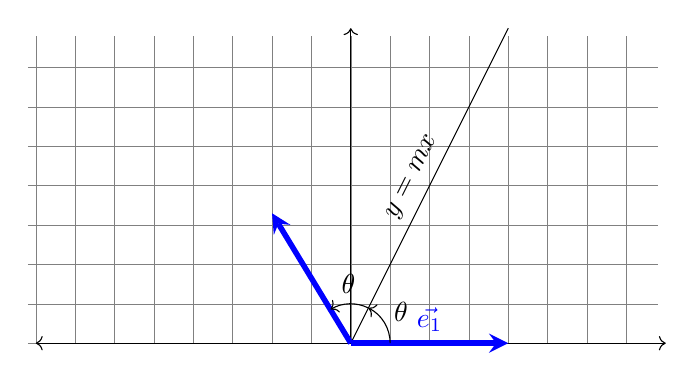
\begin{tikzpicture}
                \draw[step=.5,gray,very thin] (-4.0 - 0.1,0) grid (4.0 - 0.1, 4.0 - 0.1);
                \draw[<->] (-4.0, 0) -- (4.0, 0);
                \draw[->] (0, 0) -- (0, 4.0);
                \draw[-] (0, 0) -- (2, 4) node[midway, above, sloped]{$y= mx$ } ;
                \draw[line width=2pt,blue,-stealth] (0, 0) -- (2, 0) node[midway, above, sloped]{$\vec{e_1} $ } ;
                \draw[line width=2pt,blue,-stealth] (0, 0) -- (-1, 1.65) node[midway, above, sloped]{} ;
                \coordinate (a) at (1, 0);
                \coordinate (b) at (0, 0);
                \coordinate (c) at (1, 2);
                \pic [draw, ->, "$\theta$", angle eccentricity=1.5] {angle = a--b--c};
                \coordinate (a) at (1, 2);
                \coordinate (b) at (0, 0);
                \coordinate (c) at (-.45, .75);
                \pic [draw, ->, "$\theta$", angle eccentricity=1.5] {angle = a--b--c};
            \end{tikzpicture}
        \end{center}
        As we can see this is a counter clockwise rotation of $2\theta $ and thus we know that the vfirst column of the matrix must be 
        \[
            \mat{ \cos{2\theta }  \\ \sin{2\theta}  }
        \]
        we know that $\sin \left( 2\theta  \right) = \sin \left( \theta  + \theta  \right) = 2\sin \left( \theta \right) \cos \left( \theta \right) $ and that $\cos \left( 2\theta  \right) = \cos ^2  \left( \theta \right)  - \sin^2  \left( \theta \right) $ or equivalently 
        \[
        \mat{ \cos ^2  \left( \theta \right)  - \sin^2  \left( \theta \right) \\ 2\sin \left( \theta \right) \cos  \left( \theta \right) } 
        \]
        But we know from above that $\sin \left( \theta \right) = \frac{m}{\sqrt{m^2  + 1} }$ and $\cos  \left( \theta \right) = \frac{1}{\sqrt{m^2  + 1} }$ so we can say that $\cos ^2  \left( \theta \right)  - \sin^2  \left( \theta \right) = \frac{1 - m^2 }{m^2  + 1}$ and that $2\sin \left( \theta \right) \cos  \left( \theta \right) = \frac{2m}{m^2  + 1}$ and so so the first column is 
        \[
        \mat{ \frac{1 - m^2 }{m^2  + 1} \\ \frac{2m}{m^2  + 1} }    
        \]
        Now we'll see what happens to $\vec{e_2} $ 
        \begin{center}
            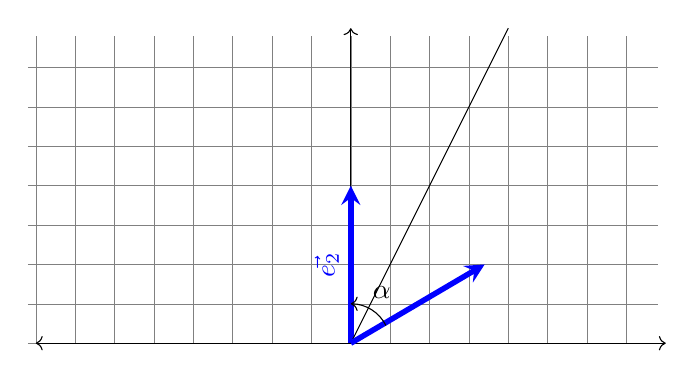
\begin{tikzpicture}
                \draw[step=.5,gray,very thin] (-4.0 - 0.1,0) grid (4.0 - 0.1, 4.0 - 0.1);
                \draw[<->] (-4.0, 0) -- (4.0, 0);
                \draw[->] (0, 0) -- (0, 4.0);
                \draw[line width=2pt,blue,-stealth] (0, 0) -- (0, 2) node[midway, above, sloped]{$\vec{e_2} $ } ;
                \draw[-] (0, 0) -- (2, 4) node[midway, above, sloped]{} ;
                \draw[line width=2pt,blue,-stealth] (0, 0) -- (1.7, 1) node[midway, above, sloped]{} ;
                \coordinate (c) at (0, 1);
                \coordinate (b) at (0, 0);
                \coordinate (a) at (1, .5);
                \pic [draw, ->, "$\alpha $", angle eccentricity=1.5] {angle = a--b--c};
            \end{tikzpicture}
        \end{center}
        But this time notice that $\alpha = 2 \cdot \left( \frac{\pi }{2} - \theta  \right) = \pi  - 2\theta $ and thus 
        \begin{align*}
            \sin \left( \pi  - 2\theta  \right) &= \sin \left( \pi  \right) \cos  \left( 2\theta  \right)  - \cos  \left( \pi  \right) \sin \left( 2\theta  \right)  \\
            &= 2\sin \left( \theta \right) \cos  \left( \theta \right) 
            \intertext{as for cosine}
            \cos  \left( \pi  - 2\theta  \right) &= \cos  \left( \pi  \right) \cos  \left( 2\theta  \right) + \sin \left( \pi  \right) \sin \left( 2\theta  \right)  \\
            &= \sin^2  \left( \theta \right)  - \cos ^2  \left( \theta \right)  \\
        \end{align*}
        And thus our total matrix is 
        \[
        \begin{bmatrix}
        	\frac{1 - m^2 }{m^2  + 1} &  \frac{-2m}{m^2  + 1} \\
        	\frac{2m}{m^2 + 1 } &  \frac{m^2  - 1}{m^2  + 1}
        \end{bmatrix}
        \]
        
\end{itemize}

% section tutorial_7 (end)

% section lecture_2 (end)

% chapter week_11 (end)

\chapter{Week 12}%
\label{chp:week_12}
% chapter week_12

\section{Lecture 1 Week 12}%
\label{sec:lecture_1_week_12}
% section lecture_1

Remember from last week, if we have that $X= \left[ T \right]_{\mathcal{C}} $ that that means for all $\vec{v} $ 
\[
\left[ T\left(\vec{v} \right) \right]_{\mathcal{C}} = X\left[ \vec{v}  \right]_{\mathcal{C}} 
\]
Specificially if $\vec{v} = \alpha \vec{c_1}  + \beta \vec{c_2} $ then we know
\[
\left[ T\left(\alpha \vec{c_1}  + \beta \vec{c_2} \right) \right]_{\mathcal{C}} = X\mat{ \alpha  \\ \beta  } 
\]

And so we recall that 
\[
\left[ \vec{v}  \right]_{\mathcal{C}} \xrightarrow{X} \left[ T\left(\vec{v} \right) \right]_{\mathcal{C}} 
\]

also if $Y= \left[ T\right]_{\mathcal{E}} $ then we know
\[
\left[ \vec{v}  \right]_{\mathcal{E}} \xrightarrow{Y} \left[ T\left(\vec{v} \right) \right]_{\mathcal{E}} 
\]

Thus if we only know what $X$ is and we want to find out what what $\left[ T\left(\vec{v} \right) \right]_{\mathcal{E}} $ then our process to do so would look like
\begin{equation*}
    \left[ \vec{v}  \right]_{\mathcal{E}} \xrightarrow{A^{-1} } \left[ \vec{v}  \right]_{\mathcal{C}} \xrightarrow{X} \left[ T\left(\vec{v} \right) \right]_{\mathcal{C}} \xrightarrow{A} \left[ T\left(\vec{v} \right) \right]_{\mathcal{E}} 
\end{equation*}

Thus we've determined the following
\begin{equation*}
    AXA^{-1} \left[ \vec{v}  \right]_{\mathcal{E}} = \left[ T\left(\vec{v} \right) \right]_{\mathcal{E}}        
\end{equation*}

Thus we conclude $AXA^{-1} = \left[ T \right]_{\mathcal{E}} $ 

\begin{defn}[Similar Matricies]\index{Similar Matricies}\label{defn:similar_matricies}
    We say that two matricies $A$ and $B$ are \hlnotea{similar } denoted $A \sim B$. If $A$ and $B$ represent the same linear transformation but in possibly different bases. Equivalently , $A \sim B $, if there exists an invertible matrix $X$ so that 
    \[
    A= XBX^{-1} 
    \]
\end{defn}

\begin{defn}[Unit n-cube]\index{Unit n-cube}\label{defn:unit_n_cube}
    The \hlnotea{unit n-cube} is the n-dimensional cube with sides given by the standard basis vectors and lower-left corner located at the origin. That is 
    \[
        C_{n} = \left\{ \vec{x} \in \mathbb{R} ^{n} : \vec{x} = \sum_{i=1}^{n} \alpha _{i} \vec{e_{i} } \text{ for some  } \alpha_1, \ldots, \alpha_{n} \in \left[ 0,1 \right]   \right\} = \left[ 0,1 \right] ^{n} 
    \]
\end{defn}

\subsection{64}%
\label{sub:64}
% subsection 64

\begin{itemize}
    \item $T\left(\mat{ 1 \\ 0 } \right)= \mat{ 1 \\ \frac{1}{2} } $ we can see that $T\left(\vec{e_2} \right) = \mat{ \frac{1}{2} \\ 1 } $ thus a matrix for $T$ is
        \[
        T = \mat{ 1 & \frac{1}{2} \\ \frac{1}{2} & 1 }
        \]
    \item To find the volume of the image of the unit-square under $T$ we will subtract area from a square with length $\frac{3}{2}$ after some observation we recognize that the area we are subtracting is 6 squares of side length $\frac{1}{2}$ which is a total volume of $\frac{6}{4}$ then our answer is 
        \begin{align*}
            \left( \frac{3}{2} \right) ^2  - \frac{6}{4} &= \frac{3}{4} \\ 
        \end{align*}
\end{itemize}

% subsection 64 (end)

\begin{defn}[Determinant]\index{Determinant}\label{defn:determinant}
    The \hlnotea{determinant } of a linear transformation $X : \mathbb{R} ^{n}  \to \mathbb{R} ^{n}  $ is the oriented volume of the image of the unit n-cube . The determinant of a square matrix is the determinant of it's induced transformation 
\end{defn}

\begin{eg}
    We know that the determinant of $T$  should be positive since we can move $T\left(\vec{e_1} \right) $ and $T\left(\vec{e_2} \right) $ are positively oriented $\left\{ \mat{ 1 \\ \frac{1}{2} } , \mat{ \frac{1}{2} \\ 1 }  \right\} $ so indeed the determinant is $\frac{3}{4}$ 
\end{eg}

\subsection{65}%
\label{sub:65}
% subsection 65

We already know what $C_{2} $ looks like lets see what $A\left(C_{2} \right) $ looks like.

\begin{center}
    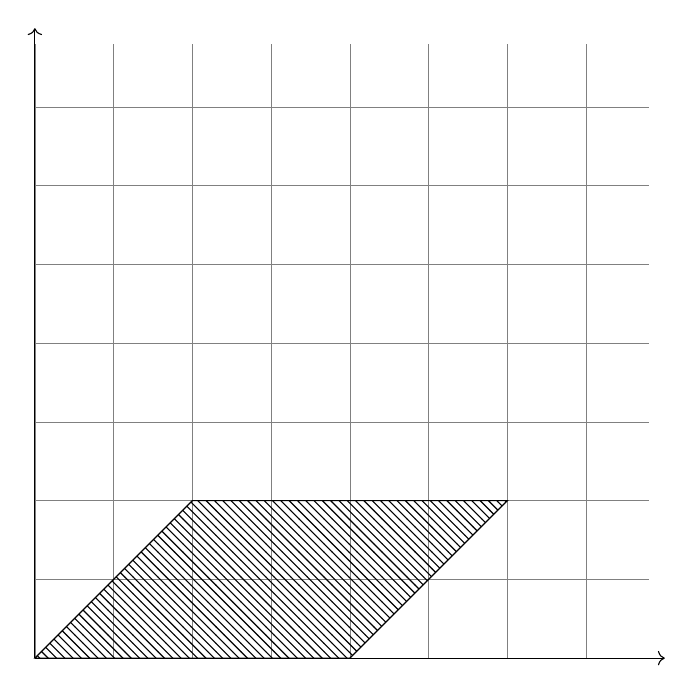
\begin{tikzpicture}[scale=2]
        \draw[step=.5,gray,very thin] (0,0) grid (4.0 - 0.1, 4.0 - 0.1);
        \draw[->] (0, 0) -- (4.0, 0);
        \draw[->] (0, 0) -- (0, 4.0);
        \draw[pattern=north west lines] (0,0) -- (1, 1) -- (3,1) -- (2,0) -- cycle;
    \end{tikzpicture}
\end{center}

We can see that the determinant should be positive and that the area is $1$ so $\mathit{det} \left(A\right) = 1$ 

% subsection 65 (end)

\subsection{66}%
\label{sub:66}
% subsection 66

We will get

\begin{center}
    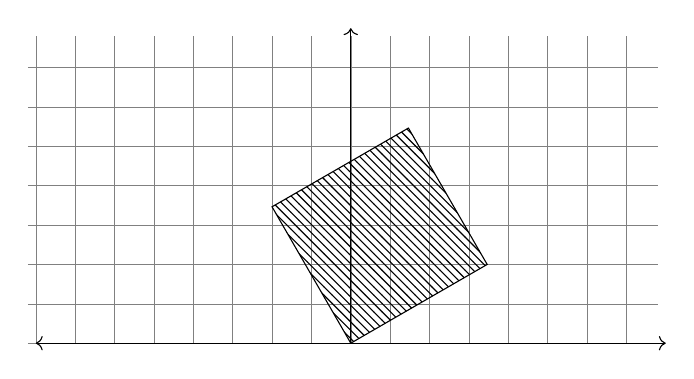
\begin{tikzpicture}
        \draw[step=.5,gray,very thin] (-4.0 - 0.1,0) grid (4.0 - 0.1, 4.0 - 0.1);
        \draw[<->] (-4.0, 0) -- (4.0, 0);
        \draw[->] (0, 0) -- (0, 4.0);   
        \draw[pattern=north west lines,rotate=30] (0,0) rectangle (2,2);
    \end{tikzpicture}
\end{center}

We observe that this doesn't modify the cube in any way so $\mathit{det} \left(R\right) = 1$ 

% subsection 66 (end)

\subsection{67}%
\label{sub:67}
% subsection 67

We can see that this just switches $\vec{e_2} \text{ and } \vec{e_1} $ so $\mathit{det} \left(F\right) = -1$ 

% subsection 67 (end)

\begin{thm}[Volume Theorem I]\index{Volume Theorem I}\label{thm:volume_theorem_i}
    For a square matrix $M$, $\mathit{det} \left(M\right) $ is the oriented volume of the parallelpiped (n-dimensional parallelogram ) given by the column vectors of $M$  
\end{thm}

\begin{thm}[Volume Theorem II]\index{Volume Theorem II}\label{thm:volume_theorem_ii}
    For a square matrix $M$,  $\mathit{det} \left(M\right) $ is the oriented volume of the parallelpiped (n-dimensional parallelogram ) given by the row vectors  of $M$.  \todo{Why???} 
\end{thm}

\begin{eg}
    Thus we know that $\mathit{det} \left(A\right) = \mathit{det} \left(A^{-1} \right) $ for example 
    \begin{align*}
        A= \mat{ \alpha  & \beta  \\ \gamma  & \delta  } && A^{-1} = \mat{ \alpha  & \gamma  \\ \beta  & \delta  } 
    \end{align*}
    
\end{eg}

\subsection{68}%
\label{sub:68}
% subsection 68

Well the columns of the matrix $M$ are $T\left(\vec{e_{i} } \right) $ and so if we look at linear combinations of those vectors where the coefficients are elements of the set $\left[ 0,1 \right] $ 

% subsection 68 (end)

\begin{remark}
    Let $\vec{v} \in C_{n} $ then there exists $\alpha _{1}, \alpha _{2}, \ldots, \alpha _{k - 1} \alpha _{k} \in \left[ 0,1 \right] $ such that $\vec{v} = \alpha _{1}\vec{e} _{1}  +  \alpha _{2}\vec{e} _{2}  +  \dotsb   +  \alpha _{k - 1}\vec{e} _{k - 1}  +  \alpha _{k}\vec{e} _{k} $ so then 
    \begin{align*}
        T\left(\vec{v} \right) &= T\left(\alpha _{1}\vec{e} _{1}  +  \alpha _{2}\vec{e} _{2}  +  \dotsb   +  \alpha _{k - 1}\vec{e} _{k - 1}  +  \alpha _{k}\vec{e} _{k} \right)   \\ 
        &= \alpha _{1}T\left(\vec{e_{1} } \right)  +   \alpha _{2}T\left(\vec{e_{2} } \right)  +   \dotsb   \alpha _{k - 1}T\left(\vec{e_{k - 1} } \right)  +   \alpha _{k}T\left(\vec{e_{k} } \right)  \\ 
    \end{align*}
    And if $k= 2$ then visually we would have
    \begin{center}
        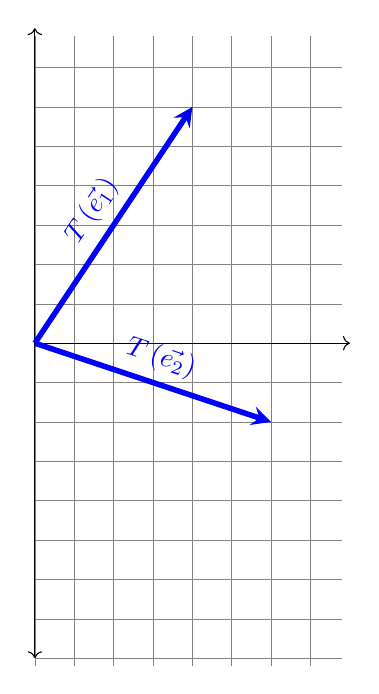
\begin{tikzpicture}
            \draw[step=.5,gray,very thin] (0,-4.0 - 0.1) grid (4.0 - 0.1, 4.0 - 0.1);
            \draw[->] (0, 0) -- (4.0, 0);
            \draw[<->] (0, -4.0) -- (0, 4.0);
            \draw[line width=2pt,blue,-stealth] (0, 0) -- (2, 3) node[midway, above, sloped]{$T\left(\vec{e_1} \right) $ } ;
            \draw[line width=2pt,blue,-stealth] (0, 0) -- (3, -1) node[midway, above, sloped]{$T\left(\vec{e_2} \right) $ } ;
        \end{tikzpicture}
    \end{center}
    Then adding the coefficients we get the parallelogram defined by $T\left(\vec{e_1} \right) , T\left(\vec{e_2} \right) $ which would look like
    \begin{center}
        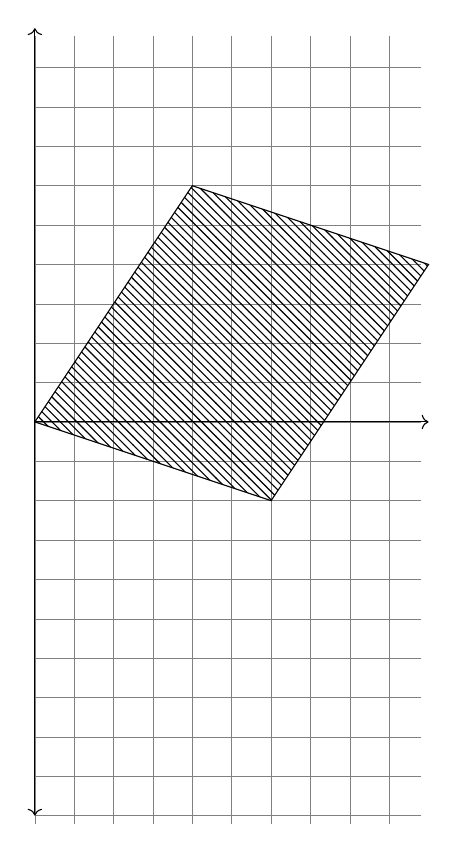
\begin{tikzpicture}
            \draw[step=.5,gray,very thin] (0,-5 - 0.1) grid (5 - 0.1, 5 - 0.1);
            \draw[->] (0, 0) -- (5, 0);
            \draw[<->] (0, -5) -- (0, 5);
            \draw[pattern=north west lines] (0,0) -- (2,3) -- (5,2) -- (3, -1) -- cycle;
        \end{tikzpicture}
    \end{center}
\end{remark}

\begin{remark}
    Let $T : \mathbb{R} ^{n}  \to \mathbb{R} ^{n}  $ we'll denote the volume of a translated unit-cube like this
    \[
    V\left(T\left(C_{n}  + \vec{b} \right) \right) \text{ for some  } \vec{b} \in \mathbb{R} ^{n} 
    \]
    Due to linearity we know
    \begin{equation*}
        V\left(T\left(C_{n} \right)  + T\left(\vec{b} \right) \right) = V\left(T\left(C_{n} \right) \right) = \mathit{det} \left(T\right) 
    \end{equation*}
\end{remark}

\begin{remark}
    Let's consider $V\left(T\left(\alpha C_{n} \right) \right) $ we know this either shrinks or stretches $C_{n} $ 
    \begin{center}
        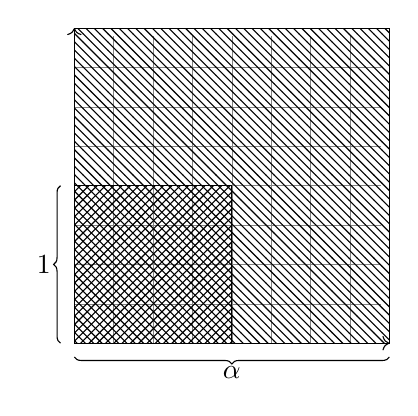
\begin{tikzpicture}
            \draw[step=.5,gray,very thin] (0,0) grid (4.0 - 0.1, 4.0 - 0.1);
            \draw[->] (0, 0) -- (4.0, 0);
            \draw[->] (0, 0) -- (0, 4.0);
            \draw[pattern=north east lines] (0,0) rectangle (2,2);
            \draw[decoration={brace,raise=5pt},decorate] (0, 0) -- node[midway, left, xshift=-5pt] {1} (0,2);
            \draw[pattern=north west lines] (0,0) rectangle (4,4);
            \draw[decoration={brace,mirror,raise=5pt},decorate] (0, 0) -- node[midway, below, yshift=-5pt] {$\alpha $ } (4, 0);
        \end{tikzpicture}
    \end{center}
    From our diagram we observe that the increase or decreasing in volume must be $\alpha ^2 $ and for the $n$ th dimension $a^{n} $thus it follows that 
    \begin{align*}
        V\left(\alpha T\left(c_{n} \right) \right) &= a^{n} V\left(T\left(C_{n} \right) \right)   \\ 
        &= a^{n} \mathit{det} \left(T\right)  \\
        &= V\left(\alpha C_{n} \right) \mathit{det} \left(T\right)  
    \end{align*}
    Thus we conclude 
    \begin{equation*}
        V\left(T\left(\alpha C_{n}  + \vec{b} \right) \right) = \mathit{det} \left(T\right) V\left(\alpha C_{n}  + \vec{b} \right) 
    \end{equation*}
\end{remark}

We'll now show that it holds for any arbitrary shape $X$ 

\begin{proof}
    Let $X$ represent some arbitrary shape (set of vectors), we know that we can represent any shape as the sum of many or infinitely many squares of varying sizes, which some of which could also be infinitely small. So $X$ consists of elements that look like $\alpha C_{n}  + \vec{b} $ for some $\alpha \in \mathbb{R} , \vec{b} \in \mathbb{R} ^{n} $. \\
    Let $T : R^{n}  \to \mathbb{R} ^{n}  $ be a linear transformation and then the image of $X$ under $T$ are the vectors $\vec{v} \in \mathbb{R} ^{n} $ that satisfy the following
    \begin{align*}
        \vec{v} &= T\left(\vec{y} \right) \text{ for some  } \vec{y} \in R^{n} \\
        &= T\left(\alpha C_{n}  + \vec{b} \right)   \\ 
        &= \alpha T\left(C_{n} \right)  + T\left(\vec{b} \right)  
    \end{align*}
    We must now find the volume of the image the which is the sum of each square we get so we have
    \todo{complete this} 
    \begin{align*}
        \sum_{i=0}^{\infty } \alpha _{i} T\left(C_{n} \right)  + T\left(\vec{b_{i} } \right)  
    \end{align*}
\end{proof}

\section{Week 12 lecture 2}%
\label{chp:week_12_lecture_2}
% section section_name

Recall previously that if we have a transformation $T : \mathbb{R} ^{n}  \to \mathbb{R} ^{n}  $ and that 
\[
V\left(T\left(\alpha C_{n}  + \left\{ \vec{b}  \right\} \right) \right) = V\left(\alpha C_{n}  + \left\{ \vec{b}  \right\} \right) \left| \mathit{det} \left(T\right)  \right| 
\]
And so we know for any shape $A$ 
\[
V\left(T\left(A\right) \right) = \left| \mathit{det} \left(T\right)  \right| V\left(A\right) 
\]


\begin{itemize}
    \item \underline{69} 
        \begin{itemize}
            \item $R_{1} = R_{2} = R_{3} = R_{4} = \frac{1}{4}$ and $R= 1$ 
            \item $M\left(R_1\right) $ has area $\frac{1}{2}$, observe.
                \begin{center}
                    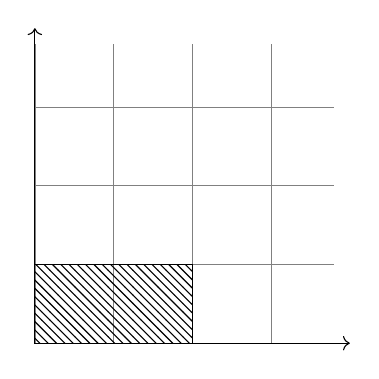
\begin{tikzpicture}[scale=2]
                        \draw[step=.5,gray,very thin] (0,0) grid (2 - 0.1, 2 - 0.1);
                        \draw[->] (0, 0) -- (2, 0);
                        \draw[->] (0, 0) -- (0, 2);
                        \draw[pattern=north west lines] (0,0) rectangle (1,0.5);
                    \end{tikzpicture}
                \end{center}
            $M\left(R_{2} \right) $ has the same area of $M\left(R_{1} \right) $ we see,
            \begin{center}
                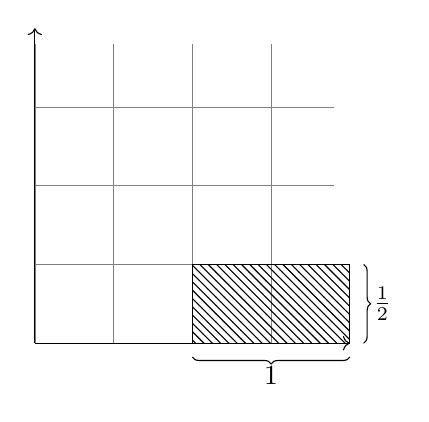
\begin{tikzpicture}[scale=2]
                    \draw[step=.5,gray,very thin] (0,0) grid (2 - 0.1, 2 - 0.1);
                    \draw[->] (0, 0) -- (2, 0);
                    \draw[->] (0, 0) -- (0, 2);
                    \draw[pattern=north west lines] (1,0) rectangle (2,.5);
                    \draw[decoration={brace,mirror,raise=5pt},decorate] (1, 0) -- node[midway, below, yshift=-5pt] {$1$ } (2, 0);
                    \draw[decoration={brace,mirror,raise=5pt},decorate] (2, 0) -- node[midway, right, xshift=5pt] {$\frac{1}{2}$ } (2, .5);
                \end{tikzpicture}
            \end{center}
            And then $M\left(R\right) $ has area 2
            \begin{center}
                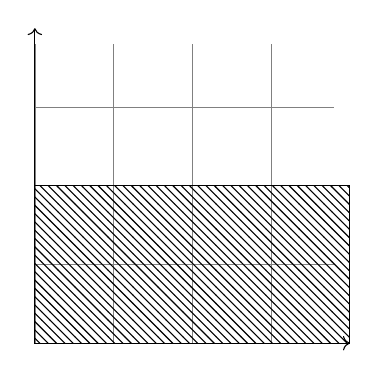
\begin{tikzpicture}[scale=2]
                    \draw[step=.5,gray,very thin] (0,0) grid (2 - 0.1, 2 - 0.1);
                    \draw[->] (0, 0) -- (2, 0);
                    \draw[->] (0, 0) -- (0, 2);
                    \draw[pattern=north west lines] (0,0) rectangle (2,1);
                \end{tikzpicture}
            \end{center}
            \item Recall $V\left(T\left(R_{2} \right) \right) = \left| \mathit{det} \left(T\right)  \right| V\left(R_{2} \right) $ and thus $2 \cdot \frac{1}{4}= \frac{1}{2}$, we know that we are just translating $T\left(R\right) $ by the vector $T\left(\vec{e_2} \right) $ and so the oriented volume is still the same as the non-translated, 2. 
            \item We start by proving the following claim. For any two linear transformations $S$, $T$ 
                \[
                V\left(S \circ T \left(R\right) \right) = \mathit{det} \left(S\right)  \cdot \mathit{det} \left(T\right)  \cdot V\left(R\right) 
                \]
            \begin{proof}
                \begin{align*}
                    V\left(S \circ T \left(R\right) \right) &= \mathit{det} \left(S\right)  \cdot V\left(T\left(R\right) \right)   \\ 
                    &= \mathit{det} \left(S\right)  \cdot \mathit{det} \left(T\right)  \cdot V\left(R\right)  
                \end{align*}
            \end{proof}
            \begin{crly}
                for any two square matricies $A,B$ 
                \[
                \mathit{det} \left(AB\right) = \mathit{det} \left(A\right) \mathit{det} \left(B\right) 
                \]
                As $A,B$ must induce a transformation 
            \end{crly}
        \end{itemize}
    \item \underline{70} 
        \begin{itemize}
            \item $E_{f} = \mat{ 0 & 1 & 0 \\ 1 & 0 & 0 \\ 0 & 0 & 1 } $ which is the transformation $f$ such that 
                \[
                f\left(\mat{ x \\ y \\ z } \right) = \mat{ y \\ x \\ z } 
                \]
                As we see this $f\left(\vec{e_1} \right) = \vec{e_2} $ and $f\left(\vec{e_2} \right) = \vec{e_1} $ and so it's negatively oriented as we can get to the standard basis by crossing once. Thus $\mathit{det} \left(f\right) = -1= \mathit{det} \left(E_{f} \right) $ 
            \item $E_{m} = \mat{ 1 & 0 & 0 \\ 0 & 1 & 0 \\ 0 & 0 & 6 }$ 
                \[
                M\left(\mat{ x \\ y \\ z } \right) = \mat{ x \\ y \\ 6z } 
                \]
                and so the unit cube becomes
                \begin{center}
                    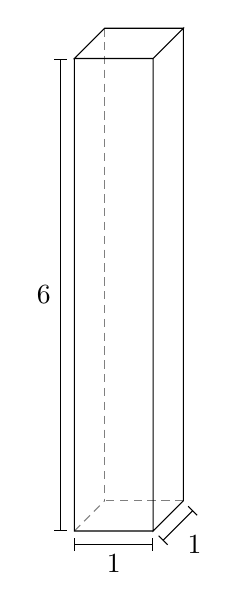
\begin{tikzpicture}
                        \pic at (0, 0) {annotated cuboid={scale=1, width=1, height=6, depth=1, units=}};
                    \end{tikzpicture}
                \end{center}
            And thus $\mathit{det} \left(M\right) = \mathit{det} \left(E_{m} \right) = 6$ 
            \item $E_{A} = \mat{ 1 & 2 & 0 \\ 0 & 1 & 0 \\ 0 & 0 & 1 }$ and so $E_{A} \mat{ x \\ y \\ z } = \mat{ x + 2y \\ y \\ z } $ so $E_{A} \vec{e_1} = \vec{e_1} , E_{A} \vec{e_2} = \mat{ 2 \\ 1 \\ 0 } , E_{A} = \vec{e_3} $ and so let we let the $z$ axis point out of the page, thus the base of the base looks like
                \begin{center}
                    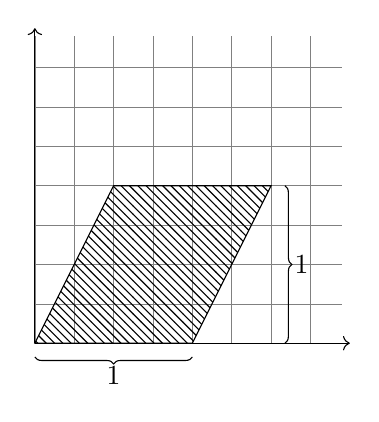
\begin{tikzpicture}
                        \draw[step=.5,gray,very thin] (0,0) grid (4.0 - 0.1, 4.0 - 0.1);
                        \draw[->] (0, 0) -- (4.0, 0);
                        \draw[->] (0, 0) -- (0, 4.0);
                        \draw[pattern=north west lines] (0,0) -- (1,2) -- (3, 2) -- (2, 0) -- cycle;
                        \draw[decoration={brace,mirror,raise=5pt},decorate] (0, 0) -- node[midway, below, yshift=-5pt] {$1$ } (2, 0);
                        \draw[decoration={brace,mirror,raise=5pt},decorate] (3, 0) -- node[midway, right, xshift=5pt] {$1$ } (3, 2);
                    \end{tikzpicture}
                \end{center}
            And so the area of the base is 1, so $\mathit{det} \left(E_{A} \right) = 1$ \\
            Notice that if we have the matrix $\mat{ 1 & \alpha  & 0 \\ 0 & 1 & 0 \\ 0 & 0 & 1 }$ and so the middle column represents
            \[
            \alpha \vec{e_1}  + \vec{e_2} 
            \]
            and that $\alpha \vec{e_1} $ gives the shift to the parallelogram which we know doesn't actually change the area of the parallelogram 
            \item $E_{f} E_{m} = \mat{ 0 & 1 & 0 \\ 1 & 0 & 0 \\ 0 & 0 & 6 }$ which takes a vector $\mat{ x \\ y \\ z } $ to $\mat{ y \\ x \\ 6z } $ which is the same as $E_{M} $ though $\vec{e_1} $ and $\vec{e_2} $ are now swapped thus it is negatively oriented so $\mathit{det} \left(f \circ m \right) = -6$ 
            \item $\mathit{det} \left(4I_{3\times 3} \right) = 4^{3} = 64$ since $\vec{e_1} \to 4\vec{e_1}, \ldots $ 
            \item We know that $W$ must look like
                \begin{gather*}
                    \begin{gmatrix}[b]
                    	1 & 0 & 0 \\
                    	0 & 1 & 0 \\
                    	0 & 0 & 1
                        \rowops
                        \mult{2}{\cdot 6} 
                        \mult{2}{\cdot 6} 
                        \swap{0}{1} 
                    \end{gmatrix}
                    \rightsquigarrow 
                    \begin{gmatrix}[b]
                    	0 & 1 & 0 \\
                    	1 & 0 & 0 \\
                    	0 & 0 & 36
                        \rowops
                        \add[2]{1}{0} 
                    \end{gmatrix}
                    \rightsquigarrow 
                    \begin{gmatrix}[b]
                    	2 & 1 & 0 \\
                    	1 & 0 & 0 \\
                    	0 & 0 & 36
                        \rowops
                        \swap{0}{1} 
                    \end{gmatrix}\\
                    \rightsquigarrow 
                    \begin{gmatrix}[b]
                    	1 & 0 & 0 \\
                    	2 & 1 & 0 \\
                    	0 & 0 & 36 
                    \end{gmatrix}
                \end{gather*}
                So we know the base has area $1$ with height $36$ so $\mathit{det} \left(W\right) = 36$ 
        \end{itemize}
\end{itemize}

\section{Tutorial 75}%
\label{sec:tutorial_75}
% section tutorial_75

\begin{itemize}
    \item Q1\\
    $\mathit{rank} \left(A\right) $ is the number of pivots in reduced row echelon form of $A$, the rank of $T$ is $\mathit{dim} \left(\mathit{range} \left(T\right) \right) $ 
    \item Q2
        \begin{enumerate}[label=\alph*)]
            \item 
                \[
                    \mat{ 1 & 0 & 0 \\ 0 & 0 & 0 }
                \]
            \item 
                \[
                    \mat{ 1 & 0 & 0 \\ 0 & 1 & 0 }
                \]
            \item We know that the number of pivots in a matrix cannot exceed the number of rows of a matrix so this is impossible
            \item 
                \[
                \mat{ 0 & 0 & 0 \\ 0 & 0 & 0 }
                \]
                We know that $\left\{ \vec{0}  \right\} $ is linearly dependent since for any $\gamma \in \mathbb{R}, \vec{0} = \gamma \vec{0} $ thus a non-trivial linear combination that yields the zero vector. 
        \end{enumerate}
    \item We'll simultaneously show a and b. \\
    If $\mathcal{L} $ is not one-to-one then we have for some $\vec{x}, \vec{y}  \in R^{n} $ such that $\vec{x} \neq \vec{y} $ that
    \begin{gather*}
        \mathcal{L}\left(\vec{x} \right) = \mathcal{L}\left(\vec{y}\right) \\
        \mathcal{L}\left(\vec{x}  - \vec{y} \right) = 0
    \end{gather*}
    But we recall that $\vec{x} \neq \vec{y} $ and so the null space is non-trivial and since the null space is a subspace we conclude that $\mathit{dim} \left(\mathit{null} \left(\mathcal{L}\left(x\right) \right) \right) \ge 1$ thus from the Rank Nullity Theorem we know that $\mathit{rank} \left(\mathcal{L} \right)  + nullity\left( \mathcal{L}  \right) = n$  and so $\mathit{rank} \left(\mathcal{L}\right)  + 1 \ge n $ thus we conclude that
    \[
    \boxed{\mathit{rank} \left(\mathcal{L} \right) < n}
    \]
    By the contrapositive of the statement we have just proven that $\mathit{rank} \left(\mathcal{L} \right) \ge n \implies \mathcal{L} \text{ is one-to-one  } $ but we know that $\mathit{rank} \left(row\left(A\right) \right) = \mathit{rank} \left(col\left( A \right)  \right) $ so then $\mathit{rank} \left(\mathcal{L} \right) \le \min\left(m, n\right) $ so the our implication changes to 
    \[
    \mathit{rank} \left(\mathcal{L} \right) = n \implies \mathcal{L} \text{ is one-to-one  } 
    \]
    This is actually a bi-implication so we have to prove the other direction. But our conclusion is that $\mathcal{L} \text{ is one-to-one  } $ if it is full rank
    \item We'll show c and d now\\
    Let $T : X \to Y $ we know that a function is onto if there exists an element in $X$ for every element in $Y$ so that it maps to it equivalently the range of $T$ is $Y$ or or we can say $T\left(X\right) = Y$ so we know
    \begin{gather*}
        image\left(\mathcal{L} \right) = R^{m} \\
        \mathit{rank} \left(\mathcal{L} \right) = m
    \end{gather*}
    So we've shown that if $\mathcal{L} $ is onto then $\mathit{rank} \left(\mathcal{L} \right) = m$ \\
    We'll show d now, remember for any $a, b \in \mathbb{R} $ one of the following is true
    \[
    a= b\lor a > b \lor a < b
    \]
    so if $\mathit{rank} \left(\mathcal{L} \right) \neq m \implies \left( \mathit{rank} \left(\mathcal{L} \right) < m \right) \lor \left( \mathit{rank} \left(\mathcal{L} \right) > m \right) $ though we know that $\mathit{rank} \left(\mathcal{L} \right) > m$ cannot be true so we know
    \[
    \text{ onto } \Leftrightarrow \mathit{rank} \left(\mathcal{L} \right) = m
    \]
    and so then 
    \[
    \text{ not-onto } \Leftrightarrow \mathit{rank} \left(\mathcal{L} \right) < m
    \]
    And finally we conclude if a function is both onto and one-to-one (bijective ) if $\mathit{rank} \left(\mathcal{L} \right) = m \land \mathit{rank} \left(\mathcal{L} \right) = n$ equivalently that is $m= n$ 
\end{itemize}

% section tutorial_75 (end)

% chapter week_12_lecture_2 (end)

% section lecture_1 (end)

% chapter week_12 (end)

\end{document}
